\documentclass[10pt]{article}
\usepackage[T1]{fontenc}
\usepackage{amsmath,amssymb,amsthm}
\usepackage[shortlabels]{enumitem}
\usepackage[english]{babel}
\usepackage[utf8]{inputenc}
\usepackage{fancyhdr}
\usepackage{bold-extra}
\usepackage{color}   
\usepackage{tocloft}
\usepackage{graphicx}
\usepackage{lipsum}
\usepackage{wrapfig}
\usepackage{cutwin}
\usepackage{hyperref}
\usepackage{lastpage}
\usepackage{multicol}
\usepackage{tikz}
\usetikzlibrary{positioning}
\usepackage{tikz-cd}
\usepackage{xcolor}
\usepackage{microtype}
\usepackage{algpseudocode}
\usepackage{biblatex}

\addbibresource{485sample.bib}

\numberwithin{equation}{section}

% some useful math commands
\newcommand{\eps}{\varepsilon}
\newcommand{\R}{\mathbb{R}}
\newcommand{\C}{\mathbb{C}}
\newcommand{\N}{\mathbb{N}}
\newcommand{\Z}{\mathbb{Z}}
\newcommand{\Q}{\mathbb{Q}}
\newcommand{\K}{\mathbb{K}}
\newcommand{\F}{\mathbb{F}}
\newcommand{\bbL}{\mathbb{L}}

\newcommand{\PubKey}{{\sf PubKey}}
\newcommand{\SecKey}{{\sf SecKey}}
\newcommand{\Enc}{{\sf Enc}}
\newcommand{\Dec}{{\sf Dec}}
\newcommand{\ord}{{\sf ord}}
\newcommand{\w}{{\sf w}}
\newcommand{\QR}{{\sf QR}}
\newcommand{\QNR}{{\sf QNR}}
\newcommand{\RNG}{{\sf RNG}}
\newcommand{\IsPrime}{{\sf IsPrime}}
\newcommand{\True}{{\sf True}}
\newcommand{\False}{{\sf False}}
\newcommand{\counter}{{\sf counter}}
\newcommand{\FW}{{\sf FW}}
\newcommand{\EJW}{{\sf EJW}}
\newcommand{\MRW}{{\sf MRW}}
\newcommand{\IntFac}{{\sf IntFac}}
\newcommand{\FindFac}{{\sf FindFac}}
\newcommand{\FB}{{\sf FB}}
\newcommand{\DLP}{{\sf DLP}}
\newcommand{\CDH}{{\sf CDH}}
\newcommand{\BreakDH}{{\sf BreakDH}}
\newcommand{\BreakElGamal}{{\sf BreakElGamal}}
\newcommand{\EXP}{{\sf EXP}}
\newcommand{\CRT}{{\sf CRT}}
\newcommand{\Sig}{{\sf Sig}}
\newcommand{\Ver}{{\sf Ver}}

\DeclareMathOperator{\GL}{GL}
\DeclareMathOperator{\id}{id}
\DeclareMathOperator{\Arg}{Arg}
\DeclareMathOperator{\Log}{Log}
\DeclareMathOperator{\PV}{PV}
\DeclareMathOperator{\sech}{sech}
\DeclareMathOperator{\csch}{csch}
\DeclareMathOperator{\ch}{char}

\algdef{SE}[SUBALG]{Indent}{EndIndent}{}{\algorithmicend\ }%
\algtext*{Indent}
\algtext*{EndIndent}

% title formatting
\newcommand{\newtitle}[4]{
  \begin{center}
	\huge{\textbf{\textsc{#1 Course Notes}}}
    
	\large{\sc #2}
    
	{\sc #3 \textbullet\, #4 \textbullet\, University of Waterloo}
	\normalsize\vspace{1cm}\hrule
  \end{center}
}

% for theorems
\newtheoremstyle{newstyle}      
{} %Aboveskip 
{-0.25pt} %Below skip
{\mdseries} %Body font e.g.\mdseries,\bfseries,\scshape,\itshape
{} %Indent
{\scshape} %Head font e.g.\bfseries,\scshape,\itshape
{.} %Punctuation afer theorem header
{ } %Space after theorem header
{} %Heading

\theoremstyle{newstyle}

\newtheorem*{prop*}{Proposition}
\newtheorem*{cor*}{Corollary}
\newtheorem*{exercise*}{Exercise}
\newtheorem*{lemma*}{Lemma}
\newtheorem*{remark*}{Remark}
\newtheorem*{exmp*}{Example}
\newtheorem*{defn*}{Definition}
\newtheorem*{thm*}{Theorem}
\newtheorem*{notation*}{Notation}
\newtheorem{thm}{Theorem}[section]
\newtheorem{fact}[thm]{Fact}
\newtheorem{cor}[thm]{Corollary}
\newtheorem{lemma}[thm]{Lemma}
\newtheorem{remark}[thm]{Remark}
\newtheorem{prop}[thm]{Proposition}
\newtheorem{defn}[thm]{Definition}
\newtheorem{claim}[thm]{Claim}
\newtheorem{axiom}[thm]{Axiom}
\newtheorem{notation}[thm]{Notation}
\newtheorem{exercise}[thm]{Exercise}
\newtheorem{exmp}[thm]{Example}
\newtheorem{algo}[thm]{Algorithm}

% new proof environment
\makeatletter
\newenvironment{pf}[1][\proofname]{\par
  \pushQED{\qed}%
  \normalfont \topsep0\p@\relax
  \trivlist
  \item[\hskip\labelsep\scshape
  #1\@addpunct{.}]\ignorespaces
}{%
  \popQED\endtrivlist\@endpefalse
}
\makeatother

% 1-inch margins
\topmargin 0pt
\advance \topmargin by -\headheight
\advance \topmargin by -\headsep
\textheight 8.9in
\oddsidemargin 0pt
\evensidemargin \oddsidemargin
\marginparwidth 0.5in
\textwidth 6.5in

\parindent 0in
\parskip 1.5ex

\setlist[itemize]{topsep=0pt}
\setlist[enumerate]{topsep=0pt}

% hyperlinks
\hypersetup{
  colorlinks=true, 
  linktoc=all,     % table of contents is clickable  
  allcolors=blue  % all hyperlink colours
}

% table of contents
\addto\captionsenglish{
  \renewcommand{\contentsname}%
    {Table of Contents}%
}
\renewcommand{\cftsecfont}{\normalfont}
\renewcommand{\cftsecpagefont}{\normalfont}
\cftsetindents{section}{0em}{2em}

\fancypagestyle{plain}{%
\fancyhf{} % clear all header and footer fields
\lhead{CO 485: Fall 2021}
\fancyhead[R]{Table of Contents}
%\headrule
\fancyfoot[R]{{\small Page \thepage\ of \pageref*{LastPage}}}
}

% headers and footers
\pagestyle{fancy}
\renewcommand{\sectionmark}[1]{\markboth{#1}{#1}}
\lhead{CO 485: Fall 2021}
\cfoot{}
\setlength\headheight{14pt}

%\setcounter{section}{-1}

\begin{document}

\pagestyle{fancy}
\newtitle{CO 485}{The Mathematics of Public Key Cryptography}{Koray Karabina}{Fall 2021}
\rhead{Table of Contents}
\rfoot{{\small Page \thepage\ of \pageref*{LastPage}}}

\tableofcontents
\vspace{1cm}\hrule
\fancyhead[R]{\nouppercase\rightmark}
\newpage 
\fancyhead[R]{Section \thesection: \nouppercase\leftmark}

\section{Introduction}

\subsection{What is Cryptography?}
Cryptography is the science of securing information and communication in the presence of attackers. As an example, cryptography helps clients do online banking safely. In a typical online banking application, clients are connected to their banks through a wireless channel which can be observed or controlled by attackers. In particular, we assume that attackers can read, modify, delete exchanged messages, and inject new messages into the channel. How can we secure a channel between two parties if they have never met before?

This scenario motivates the fundamental goals of cryptography.
\begin{itemize}
    \item The first goal is {\bf confidentiality}. Confidentiality ensures that only authorized parties can access or see the data. Attackers should not be able to extract the real content of the data even though they can read or steal packages exchanged in the channel. We would like to keep our banking passwords to ourselves.
    \item The second goal is {\bf message authentication}. Message authentication, also known as data origin authentication, assures that parties can verify the source of the received messages. When we receive a message, which is claimed to be sent from our bank, we have to make sure it has indeed been sent from our bank.
    \item The third goal is {\bf data integrity}. Data integrity assures that data cannot be altered by unauthorized or unknown means. When we are willing to pay 1,500 CAD for a new laptop, and commit to this transaction at a time, we have to make sure that this transaction cannot be modified as a 15,000 CAD worth transaction at a later time.
    \item Finally, the fourth goal is {\bf non-repudiation} which prevents communicating parties from falsely denying their actions. Once we commit to a 1,500 CAD transaction, then we should not be able to break our commitment.
\end{itemize}

There is a variety of cryptographic techniques that help achieve the fundamental goals of cryptography. As a high-level overview, encryption algorithms help achieve confidentiality; digital signature schemes help achieve authentication and non-repudiation; message authentication codes help achieve data integrity.

{\bf Public key cryptography.} Now, let’s go back to our online banking scenario. Before the communication between the client and the bank starts, the bank generates a public key, secret key pair $(\PubKey, \SecKey)$. The key $\PubKey$ is public in the sense that it is known to everyone including attackers. The key $\SecKey$ is secret in the sense the bank is the only party that knows it. After the bank generates its key pair $(\PubKey, \SecKey)$, the bank visits a certification authority. The certification authority issues a certificate to validate the public key $\PubKey$, and its ownership by the bank.

One can view the public key certificate of a website by clicking on the lock icon displayed on the 
web browser. This should display a certificate viewer, where one can click on the ``Details'' tab. 
The certificate includes information about the website, the certification authority (also known as the verifier), the validity period of the certificate, the website’s public key, and the certification authority’s signature. The public key and the signature are long sequences of hexadecimal characters.
Of course, we do not see any trace of the secret key in the certificate.

For a concrete example, the Bank of Canada is using the RSA public key cryptosystem, and its public key consists of two integers $N$ and $e$, which are called the {\bf public modulus} and the {\bf public exponent}, respectively. The certificate encodes these two integers (see \href{https://en.wikipedia.org/wiki/ASN.1}{ASN.1}), and displays them using hexadecimal (base-16) representation. For decoding, one can copy and paste the encoded public key to an ASN.1 decoder. For instance, this \href{https://lapo.it/asn1js/}{ASN.1 JavaScript decoder} can be used to decode the hexadecimal and integer values of $N$ and $e$.

\begin{exercise*}
Find the public key modulus and exponent of the \href{https://uwaterloo.ca/}{University of Waterloo} and \href{https://google.ca}{google.ca}.
\end{exercise*}

We should note two important properties of the Bank of Canada’s public key values. 
Notice that $N$ is a 2048-bit composite integer, which is supposed to be very hard to factor; 
moreover, $e=2^{16}+1$ is a relatively small integer with Hamming weight 2. The first property assures the security of the system, and the second property is for efficient implementation of the protocol. We will explain these in more detail when we cover the RSA cryptosystem.

Now that we know more about public key certificates, we can summarize the sequence of steps for turning a wireless {\bf insecure} communication channel into a secure channel between a client and her bank.
\begin{enumerate}
    \item {\bf Public key generation.} The bank generates a public key and secret key pair.

    \item {\bf Signature generation.} Certificate authority issues a certificate to the bank, validating the public key and its ownership by the bank.

    \item {\bf Signature verification.} The client obtains the bank’s certificate, and verifies the certification authority’s signature on the bank’s certificate. In other words, the client authenticates the bank.

    \item {\bf Random number generation.} The client creates a random secret session key $K$.

    \item {\bf Public key encryption.} The client encrypts $K$ using the bank’s public key $\PubKey$, and sends this encrypted key to the bank.

    \item {\bf Public key decryption.} The bank decrypts the client’s ciphertext using its private key $\SecKey$, and recovers the session key $K$.

    \item {\bf Symmetric key cryptography.} The client and the bank use the shared secret key $K$ to secure and authenticate their communication, using symmetric key cryptography.

    \item {\bf Efficiency and security.} Presumably, the steps above can be performed efficiently and that attackers cannot gather any useful information about the secret key $K$, and that the communication channel stays secure.
\end{enumerate}

In this course, we will cover these steps in detail with the exception of symmetric key cryptography. 
One can read Chapter 1.1 and Chapter 1.7 in \href{https://link-springer-com.proxy.lib.uwaterloo.ca/book/10.1007/978-1-4939-1711-2}{An Introduction to Mathematical Cryptography} and Chapter 1.5 in \href{https://www-taylorfrancis-com.proxy.lib.uwaterloo.ca/books/mono/10.1201/9780429466335/handbook-applied-cryptography-alfred-menezes-paul-van-oorschot-scott-vanstone}{Handbook of Applied Cryptography} 
for introductory level texts on symmetric key cryptography.

\subsection{The RSA Cryptosystem}

\href{https://en.wikipedia.org/wiki/RSA_(cryptosystem)}{RSA} is a public key cryptosystem invented by Ron Rivest, Adi Shamir, and Leonard Adleman, and published in 1978. The RSA cryptosystem offers a public key encryption scheme and a digital signature scheme.

{\bf The RSA encryption scheme.} The RSA public key encryption scheme consists of three algorithms.
\begin{enumerate}
    \item {\bf Key generation.} The purpose of this algorithm is to generate a public key and secret key pair. The public key is a pair of integers
    \[ \PubKey = [N, e], \]
    where $N = p\cdot q$ is a product of two randomly chosen distinct primes $p$ and $q$, and 
    $e \in (1, (p-1)(q-1))$ such that
    \[ \gcd(e, (p-1)(q-1)) = 1. \]
    For ease of notation, we define $\phi = (p-1)(q-1)$ so that $\gcd(e, \phi) = 1$. As mentioned in 
    Section 1.1, $N$ and $e$ are also called the {\bf public modulus} and the {\bf public 
    exponent}, respectively. The secret key is a tuple of integers 
    \[ \SecKey = [p, q, d], \]
    where $p$ and $q$ are as chosen before, and $d$ is the multiplicative inverse of 
    $e$ modulo $\phi$. That is, 
    \[ e \cdot d \equiv 1 \pmod \phi. \]
    The integer $d$ is also known as the {\bf secret exponent}.
    
    \newpage
    {\sc Example.} The bank chooses two distinct 8-bit random primes $p = 233$ and $q = 211$. 
    Therefore, $N = p \cdot q = 49163$ and $\phi = (p-1)(q-1) = 48720$. Next, the bank 
    chooses $e = 20771$ (one can verify that $\gcd(e, \phi) = 1$). This choice of $e$ fixes 
    $d = 36971$ since $e$ and $d$ must satisfy $e \cdot d \equiv 1 \pmod \phi$. Therefore, the bank has 
    a public key and secret pair given by 
    \begin{align*}
        \PubKey &= [N, e] = [49163, 20771], \\
        \SecKey &= [p, q, d] = [233, 211, 36971].
    \end{align*}
    
    {\sc Question.} How do you choose a fixed-length prime number at random? How do you compute modular multiplicative inverses? Are these methods efficient? What does efficient mean?
    
    \item {\bf Encryption algorithm.} Let $\Z_N$ denote the set of integers modulo $N$. 
    For a given public key $\PubKey = [N, e]$, the encryption algorithm takes as input a message 
    $m$ from the message space $\Z_N$, and outputs the ciphertext $c = m^e \pmod N$ in the 
    ciphertext space $\Z_N$. We can denote this process by 
    \begin{align*}
        \Enc_{N,e} : \Z_N &\to \Z_N \\
        m &\mapsto c = m^e \pmod N,
    \end{align*}
    or simply by $\Enc(m) = m^e \mod N$ when $N$ and $e$ are clear from the context.
    
    {\sc Example.} The client obtains the bank’s public key $\PubKey = [N,e] = [49163,20771]$, 
    and encrypts her \href{https://en.wikipedia.org/wiki/Card_security_code}{Card Security Code (CSC)} $m=123$ by 
    \[ c = m^e \pmod N = 123^{20771} \pmod {49163} = 37917. \]
    
    {\sc Question.} How do you (efficiently) perform modular exponentiation?
    
    \item {\bf Decryption algorithm.} For a given public modulus $N$ and the secret exponent $d$, the decryption algorithm takes as input a ciphertext $c$ from the ciphertext space $\Z_N$, 
    and outputs the message $m = c^d \pmod N \in \Z_N$. We can denote this process by 
    \begin{align*}
        \Dec_{N,d} : \Z_N &\to \Z_N \\
        c &\mapsto m = c^d \pmod N,
    \end{align*}
    or simply by $\Dec(c) = c^d \pmod N$ when $N$ and $d$ are clear from the context.
    
    {\sc Remark.} Note that $p$ and $q$ are implicit in the decryption algorithm above. However, as we will see later, one can explicitly use them for a more efficient decryption algorithm.
    
    It should now be clear why $N$, $e$, and $d$ are called the public modulus, public exponent, and secret exponent, respectively.
    
    {\sc Example.} The bank receives the ciphertext $c=37917$ from the client, and uses its secret key to decrypt with 
    \[ m = c^d \pmod N = 37917^{36971} \pmod {49163} = 123. \]
    Observe that the bank successfully recovered the client's CSC. 
    
    {\sc Question.} Can you guarantee that the RSA decryption algorithm will always work correctly and recover the original message? Is the RSA encryption scheme secure? What does it mean for a public key encryption scheme to be secure?
\end{enumerate}\newpage 
\section{Some Number Theory}

\subsection{Modular Arithmetic}
We begin with some notation and definitions. The set of integers is denoted by $\Z$. For an 
integer $n \geq 2$, we define the sets 
\begin{align*}
    \Z_n &= \{a \in \Z : 0 \leq a < n\}, \\ \Z_n^* &= \{a \in \Z_n : \gcd(a, n) = 1\}. 
\end{align*}
For example, we have 
\begin{align*}
    \Z_{15} &= \{0, 1, 2, 3, 4, 5, 6, 7, 8, 9, 10, 11, 12, 13, 14\}, \\
    \Z_{15}^* &= \{1,2,4,7,8,11,13,14\},
\end{align*}
where we exclude all multiples of $3$ and $5$ in the latter set. 
For $a, b \in \Z_n$, we define the operations 
\begin{align*}
    a \oplus b &= a + b \pmod n, \\
    a \odot b &= a \cdot b \pmod n.
\end{align*}
For instance, given $n = 15$, one can check that $11 \oplus 13 = 9$ and $11 \odot 13 = 8$. 
Most of the algebraic operations we work with in this course are modular operations, so we will simply 
write $+$ and $\cdot$ instead of $\oplus$ and $\odot$ when it is clear from the context 
whether $+$ and $\cdot$ are regular or modular operations. 
Notice that when $a, b \in \Z_n$, we have $a + b \in \Z_n$ and $a \cdot b \in \Z_n$; moreover, 
for $a, b \in \Z_n^*$, we have $a \cdot b \in \Z_n^*$. In fact, elements in $\Z_n$ and 
$\Z_n^*$ satisfy a larger set of properties, known as the group axioms, which we will 
formally define in the following definition.

\begin{defn}
A {\bf group} $(G, *)$ is a non-empty set $G$ together with a binary operation $*$ satisfying the 
following properties:
\begin{enumerate}[(1)]
    \item $G$ is {\bf closed}: For all $a, b \in G$, we have $a * b \in G$. 
    \item $G$ is {\bf associative}: For all $a, b, c \in G$, we have $(a * b) * c = a * (b * c)$. 
    \item $G$ has an {\bf identity}: There exists $e \in G$ such that $a * e = e * a = a$ for all $a \in G$.
    \item Elements in $G$ are {\bf invertible}: For all $a \in G$, there exists $a^{-1} \in G$ 
    such that $a * a^{-1} = a^{-1} * a = e$. 
\end{enumerate}
\end{defn}

As we noted before, $(\Z_n, +)$ is a group with identity $0$ and $(\Z_n^*, \cdot)$ is a group 
with identity $1$. However, $\Z_n$ is not a group with respect to multiplication 
because $0$ is not invertible, and 
$\Z_n^*$ is not a group with respect to addition because there is no identity element $0$. 

Finally, for a finite group $G$, the {\bf order} of $G$ is the number of elements in 
$G$, and is denoted by $|G|$. 

\subsection{GCD and Modular Inverses}
Proving the existence of inverses is interesting, but what about finding the inverse of a particular
element in a group? Finding inverses of elements in $(\Z_n, +)$ is easy: simply take the 
additive inverse $-a \pmod n$ of $a \in \Z$. On the other hand, finding the multiplicative 
inverse of an element in $(\Z_n^*, \cdot)$ takes some more work. In particular, we care about 
efficient algorithms to compute modular inverses because the secret exponent $d$ in the RSA 
encryption scheme (as in Section 1.2) is the multiplicative inverse of $e$ modulo $\phi$, where 
$e$ is the public key exponent and $\phi$ is the secret modulus. Fortunately, modular multiplicative
inverses can be computed using extended Euclidean type algorithms, and we describe one below. 

\begin{algo}[Modular Multiplicative Inverses]~

{\bf Input:} $n \geq 2$ and $a \in \Z_n^*$.

{\bf Output:} $b \in \Z_n^*$ such that $a \cdot b \equiv 1 \pmod n$. \vspace{0.5em}

\begin{algorithmic}[1]
\State Set the initial state $t_a = a$, $t_n = n$, $u = [u_0, u_1] = [1, 0]$, $v = [v_0, v_1] = [0, 1]$. 
\If{$t_n > t_a$} 
    \State Use the division algorithm to write $t_n = qt_a + r$ for some $q \geq 0$ and $0 \leq r < t_a$.
    \State Update the state: $t_n \gets r$, $v \gets v - q \cdot u$. 
\ElsIf{$t_a > t_n$}
    \State Use the division algorithm to write $t_a = qt_n + r$ for some $q \geq 0$ and $0 \leq r < t_n$.
    \State Update the state: $t_a \gets r$, $u \gets u - q \cdot v$. 
\EndIf 
\If{$t_n = 1$}
    \State Set $b = v_0 \pmod n$ and output $b$.
\ElsIf{$t_a = 1$}
    \State Set $b = u_0 \pmod n$ and output $b$.
\Else
    \State Go back to line 2.
\EndIf
\end{algorithmic}
\end{algo}

Notice that the input $(a, n)$ of Algorithm 2.2 assumes that $\gcd(a, n) = 1$ since $a \in \Z_n^*$. 
Therefore, on a more general input $(a, n)$ with $a \in \Z_n$, one first has to check that 
$\gcd(a, n) = 1$ is satisfied before Algorithm 2.2 can be run. We can address this nuisance with 
some minor modifications to the algorithm.

\begin{algo}[GCD and Modular Multiplicative Inverses]~

{\bf Input:} $n \geq 2$ and $0 \neq a \in \Z_n$.

{\bf Output:} $\gcd = \gcd(a, n)$, and if $\gcd = 1$, then $b \in \Z_n^*$ such that $a \cdot b \equiv 1 \pmod n$. \vspace{0.5em}

\begin{algorithmic}[1]
\State Set the initial state $t_a = a$, $t_n = n$, $u = [u_0, u_1] = [1, 0]$, $v = [v_0, v_1] = [0, 1]$. 
\If{$t_n > t_a$} 
    \State Use the division algorithm to write $t_n = qt_a + r$ for some $q \geq 0$ and $0 \leq r < t_a$.
    \State Update the state: $t_n \gets r$, $v \gets v - q \cdot u$. 
\ElsIf{$t_a > t_n$}
    \State Use the division algorithm to write $t_a = qt_n + r$ for some $q \geq 0$ and $0 \leq r < t_n$.
    \State Update the state: $t_a \gets r$, $u \gets u - q \cdot v$. 
\EndIf 
\If{$t_a = 0$}
    \If{$t_n = 1$}
        \State Set $\gcd = 1$, $b = v_0 \pmod n$ and output $(\gcd, b)$.
    \Else
        \State Set $\gcd = t_n$ and output $\gcd$. 
    \EndIf
\ElsIf{$t_n = 0$}
    \If{$t_a = 1$}
        \State Set $\gcd = 1$, $b = u_0 \pmod n$ and output $(\gcd, b)$.
    \Else
        \State Set $\gcd = t_a$ and output $\gcd$. 
    \EndIf
\Else
    \State Go back to line 2.
\EndIf
\end{algorithmic}
\end{algo}

\newpage
\begin{lemma}[Facts about Algorithm 2.3]~
\begin{enumerate}[(1)]
    \item Algorithm 2.3 terminates with $t_a = 0$ or $t_n = 0$. 
    \item $\gcd(t_a, t_n)$ is invariant throughout Algorithm 2.3.
    \item We have $u \cdot (a, n) = u_0a + u_1n = t_a$ and $v \cdot (a, n) = v_0a + v_1n = t_n$
    throughout Algorithm 2.3. 
\end{enumerate}
\end{lemma}
\begin{pf}
We leave the proof as an exercise. 
\end{pf}

\begin{thm}[Correctness of Algorithm 2.3]
Algorithm 2.3 terminates and its output is correct.
\end{thm}
\begin{pf}
By Lemma 2.4, we know that Algorithm 2.3 terminates with $t_a = 0$ or $t_n = 0$. Assume without 
loss of generality that it terminates with $t_a = 0$. In the beginning of the algorithm,
we set $t_a = a$ and $t_n = n$. Since $\gcd(t_a, t_n)$ is invariant throughout the algorithm by 
Lemma 2.4, we see that 
\[ \gcd(a, n) = \gcd(t_a, t_n) = \gcd(0, t_n) = t_n, \]
which shows that the first output $\gcd = t_n$ is correct. Furthermore, if $t_n = 1$ at the 
end of the algorithm, then Lemma 2.4 shows that 
\[ v \cdot (a, n) = v_0a + v_1n = t_n = 1, \]
and this implies that
\[ v_0 \cdot a \equiv 1 \pmod n. \]
Therefore, the second output $b = v_0 \pmod n$ is also correct, completing the proof.
\end{pf}

Algorithm 2.3 can be used to calculate the public key and secret key pair $(e, d)$ in the RSA 
encryption scheme. For a given RSA public modulus $N$ and secret modulus $\phi$, choose 
$e \in \Z_N$ and call Algorithm 2.3 with input $a = e$ and $n = \phi$. Repeat this until 
$\gcd = \gcd(e, \phi) = 1$ and then set the secret exponent as $d = b$, where $\gcd$ and $b$ are the 
outputs given by Algorithm 2.3. 

\subsection{Modular Exponentiation}
Let $e$ and $n\geq 2$ be integers. Let $a \in \Z_n$. Given a base $a$ and an exponent $e$, 
a modular exponential algorithm computes $a^e \in \Z_n$. We have already seen an application of modular
exponential in the RSA encryption scheme; we compute $m^e \in \Z_N$ to encrypt a message $m$, 
and compute $c^d \in \Z_N$ to decrypt a ciphertext $c$, where $e$, $d$, and $N$ are the public 
exponent, secret exponent, and public modulus, respectively. Moreover, we will see later 
that modular exponentiation is the main operation in several other cryptographic schemes. 
These include Diffie-Hellman key exchange, the elliptic curve digital signature algorithm, 
and isogeny-based cryptosystems. This gives us a lot of motivation to design and implement 
efficient modular exponentiation algorithms. 

First, we introduce some notation. We assume that exponents are positive integers unless 
otherwise stated. 
\begin{itemize}
    \item We denote the {\bf binary representation} of an $\ell$-bit integer $e = \sum_{i=0}^{\ell-1} e_i 2^i$
    where each $e_i \in \{0, 1\}$ and $e_{\ell-1} = 1$ by $(e_{\ell-1}\,e_{\ell-2}\,\cdots\,e_0)_2$. 
    Moreover, for an $\ell$-bit integer $e$, we define 
    \[ e[i : j]_2 := (e_i\,e_{i-1}\,\cdots\,e_j)_2 = \sum_{k=j}^i e_k 2^{k-j} \]
    for $0 \leq j \leq i \leq \ell-1$. Note that $e[\ell-1 : 0]_2 = e$ and $e[i : i] = e_i$.
    \item In some of the algorithms, $e$ will be represented in a more general form using a base 
    $b \geq 2$. More specifically, we write $e = \sum_{i=0}^{\ell-1} e_i b^i$ where each 
    $0 \leq e_i < b$ and $e_{\ell-1} \neq 0$. We call this the 
    {\bf $b$-ary representation} of $e$, and denote it by $e = (e_{\ell-1}\,e_{\ell-2}\,\cdots\,e_0)_b$.
    Note that the binary representation of $e$ is obtained by setting $b = 2$. 
    \item One may further relax the condition $0 \leq e_i < b$ and allow for a more general 
    digit set $D$ for the $e_i$ \cite{10.1145/322344.322355}. To be more specific, if $e$ can be written as 
    \[ e = \sum_{i=0}^{\ell-1} e_i b^i \]
    where each $e_i \in D$ for a digit set $D$, then we will still denote $e = (e_{\ell-1}\,e_{\ell-2}\,\cdots\,e_0)_b$ and extend our notation $e[i : j]_2$ to 
    \[ e[i : j]_b = (e_i\,e_{i-1}\,\cdots\,e_j)_b = \sum_{k=j}^i e_k b^{k-j}. \]
    If the base $b$ is clear from the context, we can drop it and simply write $e[i : j]$. 
    \item The complexity of some algorithms will depend on the {\bf weight} of the $b$-ary 
    representation of $e$ (the number of indices $i$ with $e_i \neq 0$), which we will denote by 
    $\w_b(a)$. 
    \item Digit sets may contain negative digits, and it will be convenient to denote a negative 
    digit $-d$ by $\overline{d}$. 
\end{itemize}

\begin{exmp}
The $2^w$-ary representations of $20771$ for $w = 1, 2, 3, 4$ are 
\begin{align*}
    20771 &= (1\,0\,1\,0\,0\,0\,1\,0\,0\,1\,0\,0\,0\,1\,1)_2 \\
    &= (1\,1\,0\,1\,0\,2\,0\,3)_4 \\
    &= (5\,0\,4\,4\,3)_8 \\
    &= (5\,1\,2\,3)_{16}
\end{align*}
A binary representation of $20771$ using the digit set $D = \{0, 1, \overline1, 3, \overline3\}$ 
and a $4$-ary representation of $20771$ using the digit set $D = \{1, \overline1, 3, \overline3\}$ are given by 
\begin{align*}
    20771 &= (1\,0\,0\,\overline3\,0\,0\,0\,1\,0\,0\,1\,0\,0\,0\,0\,3)_2 \\
    &= (1\,1\,1\,\overline3\,1\,\overline1\,\overline3\,\overline1)_4.
\end{align*}
To obtain the binary representation, we notice that 
\[ 20771 = 2^{15} - 3 \cdot 2^{12} + 2^8 + 2^5 + 3 \cdot 2^5. \]
Observe that the last representation does not use any $0$ digit and maximizes the weight 
$\w_4(e)$, whereas the second last representation is sparse with a relatively low weight $\w_2(e) = 5$.
\end{exmp}

The most widely known efficient method to perform exponentiation dates back to 200 BC and is called the 
{\bf square and multiply method}. Brauer \cite{bams/1183502136} generalized the square and multiply method using $b = 2^w$
representations of integers, where a set of elements $T = \{a_i = a^i : 1 \leq i < 2^w\}$ is 
precomputed and stored. We present this method in the following algorithm. The parameter 
$w$ used in the algorithm is also called the {\bf window size} because we iterate through $w$ 
bits at a time and we imagine placing (and moving) a window of size $w$ on the binary 
representation of the exponent. 

\begin{algo}[$2^w$-ary Square and Multiply Method]~

{\bf Input:} $w \in \Z$, $w \geq 1$, $b = 2^w$, $e = (e_{\ell-1}\,e_{\ell-2}\,\cdots\,e_0)_b$, 
$0 \leq e_i < 2^w$, $a \in \Z_n$, $n \in \Z$, $n \geq 2$.

{\bf Output:} $a^e \in \Z_n$. \vspace{0.5em}

\begin{algorithmic}[1]
\State $a_1 \gets a$, $a_i \gets a_{i-1} \cdot a$ for $2 \leq i \leq 2^w$ \Comment{we can ignore this step when $w = 1$}
\State $t \gets 1$
\For{$i = \ell-1$ {\bf to} 0 {\bf by} $-1$}
    \State $t \gets t^{2^w}$ \Comment{this step requires $w$ successive squaring operations}
    \If{$e_i \neq 0$}
        \State $t \gets t \cdot a_{e_i}$ \Comment{the multiply step; if $w = 1$, then $a_{e_i}$ is always $a$}
    \EndIf
\EndFor
\State Output $t$. 
\end{algorithmic}
\end{algo}

\newpage
\begin{thm}[Correctness of Algorithm 2.7]
Algorithm 2.7 terminates and its output is correct.
\end{thm}
\begin{pf}
The proof follows from induction and observing that $e[\ell-1 : 0]_b = 2^w \cdot (e[\ell-1 : 1]_b) + e_0$. 
We leave the details as an exercise. 
\end{pf}

\subsection{Quadratic Residues}
We now introduce quadratic residues from number theory. This will prepare us for our next 
topics on primality testing and other cryptographic constructions such as random number generators 
and public key encryption algorithms. 

Let $p$ be an odd prime. Since the only integer $a \in \Z_p$ that does not satisfy $\gcd(a, p) = 1$ is 
$a = 0$, we have $\Z_p^* = \{1, 2, \dots, p-1\}$ and $|\Z_p^*| = p-1$. 

Recall that $\Z_p^*$ is a group under multiplication. An interesting fact in algebra states that 
there always exists an element $g \in \Z_p^*$ such that for all $c \in \Z_p^*$, there is a unique 
integer $1 \leq k \leq p-1$ such that $c = g^k$. In other words, for such an element $g$, we can write 
\[ \Z_p^* = \{g^k : 1 \leq k \leq p-1\}. \]
More generally, if a (multiplicative) group $G$ has an element such that 
\[ G = \{g^k : 1 \leq k \leq |G|-1\}, \]
then we call $G$ a {\bf cyclic group} generated by $g$, and we write $G = \langle g \rangle$. 
Equivalently, we say that $g$ is a {\bf generator} of $G$. We note that a cyclic group can 
have more than one generator, and that not every group is cyclic. Indeed, $\Z_5^* = \{1, 2, 3, 4\}$ 
and $\Z_8^* = \{1, 3, 5, 7\}$ are both groups of order $4$; we have that $\Z_5^* = \langle 2 
\rangle = \langle 3 \rangle$ is cyclic, whereas $\Z_8^*$ is not since $a^2 = 1$ for all $a \in \Z_8^*$. 

It can be shown that $\Z_n^*$ is a cyclic group if and only if $n$ is one of $2$, $4$, $p^k$, or 
$2p^k$ where $p$ is an odd prime and $k$ is a positive integer. 

For a given positive integer $n$, Euler's totient function, denoted $\phi$, counts the number of positive
integers $1 \leq a \leq n$ such that $\gcd(a, n) = 1$. That is, 
\[ \phi(n) = \#\{a \in \Z : \gcd(a, n) = 1,\, 1 \leq a \leq n\}. \]
By definition, we have $|\Z_n^*| = \phi(n)$, so it is of interest to us to compute $\phi(n)$. 
Notice that we have the following properties:
\begin{enumerate}[(1)]
    \item If $p$ is a prime and $k \geq 1$ is an integer, then $\phi(p^k) = p^k - p^{k-1}$. 
    \item If $m$ and $n$ are positive integers with $\gcd(m, n) = 1$, then 
    $\phi(m \cdot n) = \phi(m) \phi(n)$. 
\end{enumerate}
In particular, for two distinct primes $p$ and $q$, we know that $|\Z_p^*| = \phi(p) = p-1$ 
and $|\Z_q^*| = \phi(q) = q-1$. It follows that if $N = p \cdot q$, then 
\[ |\Z_N^*| = \phi(N) = \phi(p)\phi(q) = (p-1)(q-1). \]
This is exactly why we defined $\phi = (p-1)(q-1)$ in the RSA encryption scheme, where we have been 
practically working with $N$. 

We now recall some important definitions and facts about finite groups. 

\begin{prop}[Properties of Finite Groups]
Let $G$ be a finite group with identity $1$. 
\begin{itemize}
    \item For all $g \in G$, we have $g^{|G|} = 1$. 
    \item The {\bf order} of an element $g \in G$ is the smallest positive integer $s$ such that 
    $g^s = 1$, denoted by $\ord(g)$. 
    \item If $g^a = 1$ for some positive integer $a$, then $\ord(g) \mid a$. In particular, we see that 
    $\ord(g) \mid |G|$. 
    \item If $\ord(g) = s$, then 
    \[ \ord(g^a) = \frac{s}{\gcd(a, s)}. \]
    In particular, we have $\ord(g) = \ord(g^a)$ if and only if $\gcd(a, \ord(g)) = 1$. 
    \item A cyclic group $G = \langle g \rangle$ has $\phi(|G|)$ generators, and the set of 
    generators is given by 
    \[ \{g^a : \gcd(a, |G|) = 1\}. \]
    \item We have $g^a = g^b$ if and only if $a \equiv b \pmod{\ord(g)}$. 
\end{itemize}
\end{prop}

Let $p$ be a prime, and consider the linear equation 
\[ ax + b \equiv 0 \pmod p \]
for $a, b \in \Z_p$ with $a \neq 0$. This equation has a solution $x = -b \cdot a^{-1}$, and one can 
show that this solution is unique. Next, consider the quadratic equation 
\[ ax^2 + bx + c \equiv 0 \pmod p \]
where $a, b, c \in \Z_p$ with $a \neq 0$. Then we can consider two cases: either the equation 
has no solution in $\Z_p$ (for instance, take $p = 3$, $a = c = 1$, and $b = 0$), or 
it has at least one solution. Suppose we are in the second case, and let $s_1$ be a solution. Then 
we can write 
\begin{align*}
    ax^2 + bx + c &= (ax^2 + bx + c) - (as_1^2 + bs_1 + c) \\
    &= a(x^2 - s_1^2) + b(x - s_1) \\
    &= (x - s_1)(ax + as_1 + b). 
\end{align*}
This gives rise to another solution $s_2 = -(s_1 + ba^{-1}) \in \Z_p$ to the same equation. 
Therefore, we can either have $0$, $1$ (when $s_1 = s_2$), or $2$ (when $s_1 \neq s_2$) solutions in 
$\Z_p$. By setting $a = 1$, $b = 0$, and taking a non-zero $c \in \Z_p$, we conclude that 
\[ x^2 \equiv c \pmod p \]
has either no solution, or solution set $\{s, -s\}$ for some $s \in \Z_p^*$. Note that $s$ cannot 
be zero, and for $p$ an odd prime, $s$ and $-s$ are pairwise distinct. This motivates the 
definition of a quadratic residue modulo $p$. 

\begin{defn}[Quadratic Residues and Non-Residues]
Let $p$ be a prime. An element $c \in \Z_p^*$ is said to be a {\bf quadratic residue} modulo $p$ if 
the equation 
\[ x^2 \equiv c \pmod p \]
as a solution in $\Z_p^*$. If $c \in \Z_p^*$ is not a quadratic residue, we call $c$ a 
{\bf quadratic non-residue} modulo $p$. The set of all quadratic residues modulo $p$ is denoted by 
$\QR_p$, and the set of all quadratic non-residues modulo $p$ is denoted by $\QNR_p$. 
\end{defn}

The following theorem gives two characterizations of $\QR_p$. 

\begin{thm}[Characterizations of $\QR_p$]
Let $p$ be an odd prime and let $g$ be a generator of $\Z_p^*$. Let $c = g^k$ for some $1 \leq k 
\leq p-1$.
\begin{enumerate}[(1)]
    \item We have $c \in \QR_p$ if and only if $k$ is even. 
    \item We have $c \in \QR_p$ if and only if $c^{(p-1)/2} = 1$ (Euler's criterion). 
\end{enumerate}
\end{thm}
\begin{pf}
To prove (1), suppose that $c \in \QR_p$. By definition, there exists $x \in \Z_p^*$ such that 
$c = x^2 = g^{2\alpha}$, where the last equality follows because $g$ is a generator of 
$\Z_p^*$. Setting $k = 2\alpha$ proves the forward direction. For the converse, let $k$ be even. 
Then we can write $c = g^k = g^{2\alpha} = x^2$ for $x = g^\alpha$, finishing the proof of (1). 
The proof of (2) follows from (1) and Proposition 2.9, and we leave it as an exercise.
\end{pf}

Euler's criterion in Theorem 2.11 can be used to test whether an element $c \in \Z_p^*$ 
is in $\QR_p$ for an odd prime $p$. \newpage 
\section{Primality Testing}

\subsection{Motivation for Primality Testing}
The key generation algorithm in the RSA encryption scheme requires us to generate two large primes $p$
and $q$ to form the public modulus $N = pq$. How large should these primes be? We have seen that 
some of the currently used public key certificates have a $2048$-bit RSA modulus $N$, which would 
require us to generate two $1024$-bit primes; we want $p$ or $q$ to be of the same size for 
security reasons. 

Suppose that we would like to generate an $\ell$-bit prime $p$. Moreover, suppose that we 
have two magic boxes $\RNG$ and $\IsPrime$. Every time we use $\RNG$, it gives us a random bit, 
or a sequence of random bits. We may have to initiate $\RNG$ with some (short but random) seed. 
Therefore, using $\RNG$ nets us a random $\ell$-bit integer $p$. Next, we provide our random integer $p$
to $\IsPrime$, which tells us $\True$ if $p$ is prime and $\False$ otherwise. We repeat this 
process until the output of $\IsPrime$ is $\True$, as depicted in the following diagram. 

\begin{center}
% https://tikzcd.yichuanshen.de/#N4Igdg9gJgpgziAXAbVABwnAlgFyxMJZARgBoAGAXVJADcBDAGwFcYkQAdDuAM2C54AjCAA9gAJQByAcQC+skLNLpMufIRQAmCtTpNW7NIuUgM2PASIBmHTQYs2iTtz4DhYgJJwACgCcsALYw8sYq5upEACy2eg7sXLzAACq+rApKYWqWKDbEuvYGTgl8AGJMcMGhpqoWGsjkMQWOIIq6MFAA5vBEoDy+EAFIDSA4EEjEGSB9A+M0o0iak9ODiNojY4iRS-0ra-OIVtszm3Mb5EcrAKynQ3b6zVw4MCI4wBXt6ZSyQA
\begin{tikzcd}
{} \arrow[r, "\text{seed}"] & {\fbox{\RNG}} \arrow[r] & p \arrow[r] & {\fbox{\IsPrime}} \arrow[d] \arrow[r] & \sf{True} \\
                            &                           &             & \sf{False} \arrow[llu]                  &          
\end{tikzcd}
\end{center}

Defining the number of primes not exceeding $L$ as $\pi(L)$ and assuming that the primes are 
randomly distributed in any given interval, we would expect to query $\IsPrime$ about 
$2^{\ell-1}/(\pi(2^\ell) - \pi(2^{\ell-1}))$ times before we have an affirmative answer on the primality
of $p$. The Prime Number Theorem tells us that $\pi(L) \approx L/\ln L$, so we would expect to 
try approximately $\ln 2^\ell$ random integers before obtaining a prime $p$. In particular, 
this means that we would run $710$ primality tests before generating a $1024$-bit prime. We can 
reduce this number in half by trying only the odd numbers, but it is still critical that we find 
efficient implementations of $\RNG$ and $\IsPrime$. This week, we will focus on $\IsPrime$. 

\subsection{A Basic Primality Test}
Let $n$ be a positive integer. If $n$ is prime, then it only has the factors $1$ and $n$, which we call 
the trivial factors of $n$. On the other hand, if $n$ is composite, then it has factors 
$n_1 \leq n_2$ with $n_1 \leq \sqrt n$. In other words, a positive integer $n \geq 2$ is prime if and 
only if it is not divisible by any integer between $2$ and $\sqrt n$. 

This observation gives us a basic primality testing algorithm. For an integer $n \geq 2$ as input, 
compute $n \pmod k$ for all integers $2 \leq k \leq \sqrt n$. If no such $k$ exists or 
$n \pmod k$ is non-zero for all $k$, then output $\True$; otherwise, there is some $k$ such that 
$n \pmod k$ is zero, in which case we output $\False$. 

This algorithm can be very quick to identify $n$ as a composite number if $n$ has a small divisor. 
However, what if our input $n$ is composite with only two prime divisors $p \approx q$? 
What if $n$ is prime (which is exactly what we are trying to determine)? In such cases, 
we would have to compute $n \pmod k$ approximately $\sqrt n$ times. To generate a 
$1024$-bit prime, we would need to run the Euclidean division algorithm about $2^{512}$ times. 
If we run this algorithm on a $4.7$ GHz computer and assume that Euclidean division can be 
computed in $1$ clock cycle, then we would expect to wait $2^{512}/(4.7 \times 10^9)$ seconds, 
or about $10^{137}$ years. This is clearly infeasible for our purposes. Fortunately, 
more efficient primality testing algorithms exist. 

\subsection{Fermat Primality Test}
Let $n \geq 2$ be a positive integer. If we can find an integer $1 \leq a \leq n-1$ such that 
$\gcd(a, n) > 1$, then we are guaranteed that $n$ is composite. However, what if the integer 
$1 \leq a \leq n-1$ satisfies $\gcd(a, n) = 1$? Then we either have $a^{n-1} \not\equiv 1 \pmod n$ 
or $a^{n-1} \equiv 1 \pmod n$. In the first case, we can conclude that $n$ is composite because 
if $n$ were prime, then $a^{n-1} \equiv 1 \pmod n$ for all $1 \leq a \leq n-1$ by Fermat's Little 
Theorem. However, in the second case, we cannot deduce whether $n$ is composite or prime. 
For example, we have $2^{340} \equiv 1 \pmod{341}$, but $n = 341 = 11 \cdot 31$ is not prime. 
This discussion motivates the definition of a Fermat witness and Fermat liar for the compositeness of $n$.

\begin{defn}
Let $n \geq 2$ and $1 \leq a \leq n-1$ be positive integers.
\begin{itemize}
    \item The integer $a$ is said to be a {\bf Fermat witness} for the compositeness of $n$ if it satisfies
    $\gcd(a, n) = 1$ and $a^{n-1} \not\equiv 1 \pmod n$. 
    \item The integer $a$ is said to be a {\bf Fermat liar} for the compositeness of $n$ if it satisfies 
    $\gcd(a, n) = 1$ and $a^{n-1} \equiv 1 \pmod n$. 
\end{itemize}
\end{defn}

We saw that $a = 2$ is a Fermat liar for the compositeness of $n = 341$ since $\gcd(2, 341) = 1$
and $2^{340} \equiv 1 \pmod{341}$. On the other hand, $a = 3$ is a Fermat witness for the compositeness
of $n = 341$ since $\gcd(3, 341) = 1$ and $3^{340} \equiv 56 \not\equiv 1 \pmod{341}$. 

We are now ready to present the Fermat primality test, where we hope that the number of Fermat liars 
is relatively low so that we can quickly find a Fermat witness for a composite integer $n$. 
If we cannot find a Fermat witness for the compositeness of $n$ after $r$ iterations, 
then we will conclude that $n$ is {\it probably} prime. We cannot say for sure that $n$ is prime 
since it is possible that $n$ is composite but no Fermat witness is found within $r$ iterations.

\begin{algo}[Fermat Primality Test]~

{\bf Input:} A positive integer $n \geq 2$ and a positive integer $r$. 

{\bf Output:} One of ``$n$ is composite'' or ``$n$ is probably prime''; the 
success probability is controlled by the input parameter $r$, the number of 
iterations. 
\begin{enumerate}
    \item {\bf for $i = 1$ to $r$ do:}
    \begin{itemize}
        \item Pick a random integer $1 < a < n-1$. 
        \item Compute $\gcd = \gcd(a, n)$. 
        \item {\bf if $\gcd > 1$:}
        \begin{itemize}[$\circ$]
            \item Output ``$n$ is composite'' and exit.
        \end{itemize}
        {\bf else:}
        \begin{itemize}[$\circ$]
            \item Compute $a^{n-1} \in \Z_n$. 
            \item {\bf if $a^{n-1} \neq 1$:}
            \begin{itemize}[--]
                \item Output ``$n$ is composite'' and exit ($a$ is a Fermat witness).
            \end{itemize}
        \end{itemize}
    \end{itemize}
    \item Output ``$n$ is probably prime'' and exit (after $r$ iterations).
\end{enumerate}
\end{algo}

It is clear that if the input $n$ to the Fermat primality test is prime, then the output 
will always be ``$n$ is probably prime'', as expected. Moreover, if the Fermat primality test 
outputs ``$n$ is composite'', then $n$ is always composite. However, as we noted above, the Fermat 
primality test can output ``$n$ is probably prime'' even when $n$ is composite. Ideally, we want 
to ensure that when the input $n$ is composite, then the probability that the algorithm will 
output ``$n$ is probably prime'' is small. This probably heavily depends on the density of Fermat 
witnesses for a composite number $n$. The good news is that the existence of a Fermat witness for a 
composite $n$ implies that at least half of the elements in $\Z_n^*$ are Fermat witnesses, as we 
shall see in the following theorem.

\begin{thm}
Let $n$ be a positive integer for which there is at least one Fermat witness. Then at least 
half of the elements in $\Z_n^* = \{a \in \Z_n : \gcd(a, n) = 1\}$ are Fermat witnesses. 
\end{thm}
\begin{pf}
Let $a \in \Z_n^*$ be a Fermat witness for the compositeness of $n$. If there is no Fermat liar in 
$\Z_n^*$, then the result holds trivially. Now, let $b_i \in \Z_n^*$ be pairwise distinct 
Fermat liars for $1 \leq i \leq s$. It suffices to show that $ab_i$ are pairwise distinct 
Fermat witnesses. First, note that $ab_i \in \Z_n^*$ since $\Z_n^*$ is a multiplicative group. 
Moreover, the $ab_i$ are pairwise distinct because $ab_i \equiv ab_j \pmod n$ would imply that 
$b_i \equiv b_j \pmod n$ by multiplying both sides by $a^{-1} \in \Z_n$. Finally, we have 
\[ (ab_i)^{n-1} \equiv a^{n-1} b_i^{n-1} \equiv a^{n-1} \not\equiv 1 \pmod n, \]
so $ab_i$ is a Fermat witness, finishing the proof. 
\end{pf}

The above theorem implies that if there is at least one Fermat witness for a composite $n$, then 
the Fermat primality test would fail with probability at most $1/2^r$. This is because for 
composite $n$, the probability that $\gcd(a, n) = 1$ and that $a$ is not a Fermat witness is at 
most $1/2$. 

Unfortunately, there are composite numbers $n$ with no Fermat witnesses. 
In other words, $a^{n-1} \equiv 1 \pmod n$ holds for all $a \in \Z_n^*$. Such an integer $n$ 
is known as a \href{https://en.wikipedia.org/wiki/Carmichael_number}{Carmichael number}, with the smallest one being $561$. There are 
infinitely many Carmichael numbers, and the number of Carmichael numbers less than $n$ is 
estimated to be about $n^{2/7}$ for sufficiently large $n$. In particular, the Fermat primality 
test will fail to output the correct answer unless we happen to choose $1 < a < n-1$ with 
$\gcd(a, n) > 1$ in one of the iterations. 

\subsection{Solovay-Strassen Primality Test}
The Fermat primality test utilizes the key equality $a^{n-1} \equiv 1 \pmod n$ which holds for all $a \in 
\Z_n^*$ when $n$ is prime. We observed a similar property, namely Euler's criterion in Proposition 2.11,
which states that if $n$ is an odd prime, then $a \in \QR_n$ if and only if $a^{(n-1)/2} = 1$. 
As one might guess, the Solovay-Strassen primality test will follow a similar approach to the 
Fermat primality test; repetitive computations of $a^{n-1} = 1$ for randomly chosen 
$a \in \Z_n^*$ will help determine if $n$ is prime or composite. Before describing the 
Solovay-Strassen primality test, we will first introduce some more definitions and algorithms 
building on our previous discussion of quadratic residues. 

\begin{defn}[Legendre symbol]
Let $p$ be an odd prime and let $a \geq 0$ be an integer. The {\bf Legendre symbol} 
$(\frac ap)$ is defined as 
\[ \left( \frac ap \right) = \begin{cases} 0 & \text{if $a \equiv 0 \pmod p$,} \\ 1 & \text{if $a \in \QR_p$,} \\ -1 & \text{if $a \in \QNR_p$.} \end{cases} \]
\end{defn}

\begin{thm}
If $p$ is an odd prime, then for all integers $a \geq 0$, we have 
\[ \left( \frac ap \right) \equiv a^{(p-1)/2} \pmod p. \]
\end{thm}
\begin{pf}
If $p$ divides $a$, then $a \equiv 0 \pmod p$, so $a^{(p-1)/2} \equiv 0 \pmod p$ and 
$(\frac ap) = 0$ by the definition of the Legendre symbol. Next, assume that $\gcd(a, p) = 1$. 
If $a \in \QR_p$, then $(\frac ap) = 1$ by definition, and $a^{(p-1)/2} \equiv 1 \pmod p$ 
by Euler's criterion. Suppose now that $a \in \QNR_p$ so that $(\frac ap) = -1$. By Proposition 
2.9, we can write $a^{p-1} \equiv 1 \pmod p$, so $a^{(p-1)/2}$ is a solution to $x^2 \equiv 1 
\pmod p$. The only two solutions to this equation are $\pm1$ as we discussed in Section 2.4. 
Since $a \in \QNR_p$, it follows from Euler's criterion that $a^{(p-1)/2} \equiv -1 \pmod p$,
completing the proof.
\end{pf}

Note that the above theorem gives us an efficient algorithm to compute the Legendre symbol. 
Now, we generalize the Legendre symbol to the Jacobi symbol $\left(\frac an\right)$ for all odd positive integers 
$n$, and present efficient algorithms to compute it. This is critical for the Solovay-Strassen 
primality test as we will declare $n$ to be composite if we can find $a \in \Z_n$ such that 
$\gcd(a, n) > 1$ or $\left(\frac an\right) \not\equiv a^{(n-1)/2} \pmod n$. 

\begin{defn}[Jacobi symbol]
Let $n$ be an odd positive integer with unique prime factorization given by 
\[ n = \prod_{i=1}^k p_i^{e_i} \]
where $p_i$ is a prime and $e_i \geq 1$ is an integer for all $1 \leq i \leq k$. 
For an integer $a \geq 0$, the {\bf Jacobi symbol} $\left(\frac an\right)$ is defined by 
\[ \left( \frac an \right) = \prod_{i=1}^k \left( \frac a{p_i} \right)^{\!e_i}, \]
where $(\frac a{p_i})$ denotes the Legendre symbol as defined above. 
\end{defn}

We noted earlier that we will declare $n$ to be composite if we can find $a \in \Z_n$ such that 
$\left(\frac an\right) \not\equiv a^{(n-1)/2} \pmod n$ in the Solovay-Strassen primality test. We already 
know how to compute $a^{(n-1)/2} \pmod p$ and $(\frac ap)$ efficiently for a prime $p$, and 
the definition of the Jacobi symbol offers an efficient way to compute $\left(\frac an\right)$. 
However, this method is not useful to us because we are trying to determine if $n$ is prime, 
whence we do not know the prime factorization of $n$. Computation number theory comes in 
handy here, and some facts about the Jacobi symbol will help us to compute the Jacobi symbol
$\left(\frac an\right)$ efficiently without needing to factor $n$.

\begin{prop}
Let $m$ and $n$ be odd positive integers. For all integers $a, b \geq 0$, we have the following properties:
\begin{enumerate}[(1)]
    \item $\left(\frac an\right) = 0$ if and only if $\gcd(a, n) > 1$. 
    \item $\left(\frac {ab}n\right) = \left(\frac an\right)\left(\frac bn\right)$. 
    \item If $a \equiv b \pmod n$, then $\left(\frac an\right) = \left(\frac bn\right)$. 
    \item $\left(\frac1n\right) = 1$. 
    \item $\left(\frac2n\right) = (-1)^{(n^2-1)/8} = \begin{cases} 1 & \text{if } n \equiv \pm1 \pmod 8, \\ -1 & \text{if } n \equiv \pm3 \pmod 8. \end{cases}$
    \item $\left(\frac mn\right) = \left(\frac nm\right) (-1)^{((m-1)/2)((n-1)/2)} = \begin{cases} -\left(\frac nm\right) & \text{if } m\equiv n \equiv 3 \pmod 4, \\ \left(\frac nm\right) & \text{otherwise.} \end{cases}$
\end{enumerate}
\end{prop}

\begin{exmp}
We can use the above facts to compute $\left(\frac{123}{5472940991761}\right)$. Indeed, we have 
\begin{align*}
    \left( \frac{123}{5472940991761} \right) &= 
    \left( \frac{5472940991761}{123} \right) = \left( \frac{70}{123} \right) 
    = \left( \frac{2}{123} \right) \left( \frac{35}{123} \right) = -\left( \frac{35}{123} \right) \\
    &= \left( \frac{123}{35} \right) = \left( \frac{18}{35} \right) = \left( \frac{2}{35} \right)
    \left( \frac{9}{35} \right) = -\left( \frac{9}{35} \right) \\
    &= -\left( \frac{35}{9} \right) = -\left( \frac{8}{9} \right) = -\left( \frac{2}{9} \right)^{\!3}
    \left( \frac{1}{9} \right) = -\left( \frac{1}{9} \right) = -1. 
\end{align*}
\end{exmp}

We now have all the computational tools we need for presenting the Solovay-Strassen primality test. 
Due to Theorem 3.5, we hope to quickly find an integer $a$ such that $\left(\frac an \right) 
\not\equiv a^{(n-1)/2} \pmod n$ for composite $n$. This is because if $n$ were prime, then
for all $a \geq 0$, we would have $\left( \frac an \right) \equiv a^{(n-1)/2} \pmod n$.
We call such an integer $a$ an Euler witness for 
the compositeness of $n$, as it certifies that $n$ is composite. If we do not find an Euler 
witness for the compositeness of $n$ after $r$ iterations, then we will conclude that 
$n$ is {\it probably} prime, as with the Fermat primality test. 

\begin{algo}[Solovay-Strassen Primality Test]~

{\bf Input:} A positive odd integer $n \geq 3$ and a positive integer $r$. 

{\bf Output:} One of ``$n$ is composite'' or ``$n$ is probably prime''; the 
success probability is controlled by the input parameter $r$, the number of 
iterations. 
\begin{enumerate}
    \item {\bf for $i = 1$ to $r$ do:}
    \begin{itemize}
        \item Pick a random integer $1 < a < n-1$. 
        \item Compute $\gcd = \gcd(a, n)$. 
        \item {\bf if $\gcd > 1$:}
        \begin{itemize}[$\circ$]
            \item Output ``$n$ is composite'' and exit.
        \end{itemize}
        {\bf else:}
        \begin{itemize}[$\circ$]
            \item Compute $\left( \frac an \right)$ and $a^{(n-1)/2} \in \Z_n$. 
            \item {\bf if $\left( \frac an \right) \not\equiv a^{(n-1)/2} \pmod n$:}
            \begin{itemize}[--]
                \item Output ``$n$ is composite'' and exit ($a$ is an Euler witness).
            \end{itemize}
        \end{itemize}
    \end{itemize}
    \item Output ``$n$ is probably prime'' and exit (after $r$ iterations).
\end{enumerate}
\end{algo}

\begin{defn}
Let $n \geq 3$ be an odd positive composite number. An integer $1 \leq a \leq n-1$ is called an 
{\bf Euler-Jacobi witness} for the compositeness of $n$ if it satisfies $\gcd(a, n) = 1$ and 
$\left( \frac an \right) \not\equiv a^{(n-1)/2} \pmod n$. Otherwise, $a$ is called an 
{\bf Euler-Jacobi liar} if it satisfies $\gcd(a, n) = 1$ and $\left( \frac an \right) 
\equiv a^{(n-1)/2} \pmod n$. 
\end{defn}

\begin{thm}[Density of Euler-Jacobi witnesses]
Let $n$ be an odd positive composite integer. Then at least half of the elements in $\Z_n^* 
= \{a \in \Z_n : \gcd(a, n) = 1\}$ are Euler-Jacobi witnesses.
\end{thm}
\begin{pf}
We leave the proof as an exercise. Show that the Euler-Jacobi liars
form a proper subgroup of $\Z_n^*$, and use the fact that the order of a subgroup divides the order 
of the group. 
\end{pf}

The above theorem implies that the Solovay-Strassen primality test will fail to output the 
correct result with probability at most $1/2^r$ since the probability that $a \in \Z_n^*$ 
is not an Euler-Jacobi witness per iteration is at most $1/2$ for composite $n$. 

We note that Theorem 3.11 is stronger than its analogous statement in Theorem 3.3 in the sense that
the number of Euler-Jacobi witnesses is bounded by $|\Z_n^*|/2$ without needing to assume the 
existence of an Euler-Jacobi witness. 

\subsection{Miller-Rabin Primality Test}

In this section, we present the Miller-Rabin primality test, where we introduce the notions of a Miller-Rabin witness and a Miller-Rabin liar. The Miller-Rabin primality test is more advantageous than the Solovay-Strassen primality test because the number of Miller-Rabin liars in $\Z_n^*$ is bounded by $(n-1)/4$, and the set of Euler-Jacobi witnesses is a subset of 
the Miller-Rabin witnesses. In particular, the wrong output is provided with probability at most 
$1/4^r$ in the case where the input $n$ is composite, where $r$ is the number of iterations. 
The Miller-Rabin primality test is widely used in practice as it is one of the simplest and 
fastest tests, while being more accurate than the Fermat and Solovay-Strassen primality tests. 

\begin{thm}
Let $p$ be an odd prime. Let $s, d \in \Z_n^*$ be elements such that $d$ is odd and 
$p - 1 = 2^s d$ with $s \geq 1$. For every $a \in \Z_p^*$, we either have 
\begin{enumerate}[(i)]
    \item $a^d \equiv 1 \pmod p$, or 
    \item $a^{2^td} \equiv -1 \pmod p$ for some $0 \leq t \leq s-1$. 
\end{enumerate}
\end{thm}
\begin{pf}
By Fermat's little theorem, we have $a^{p-1} \equiv a^{2^sd} \equiv 1 \pmod p$. Therefore, 
$a^{2^{s-1}d}$ satisfies the equation $x^2 \equiv 1 \pmod p$, which has exactly two roots 
$\pm1 \pmod p$. In other words, we either have $a^{2^{s-1}d} \equiv -1 \pmod p$ or 
$a^{2^{s-1}d} \equiv 1 \pmod p$. In the first case, we are done as (ii) holds. 
In the second case, we have $a^{2^{s-1}d} \equiv 1 \pmod p$, and if $s = 1$, then we are done as 
(i) holds. If $s > 1$, we can repeat the same process and either obtain $a^{2^td} \equiv -1 \pmod p$
for some $0 \leq t \leq s-1$ along the way, or we would have to have $a^d \equiv 1 \pmod p$, 
which completes the proof. 
\end{pf}

\begin{defn}
Let $n$ be an odd positive composite integer such that $n-1=2^sd$ for some positive integer $s$ and an odd integer $d$. An element $a\in \Z_n^*$ is called a {\bf Miller-Rabin witness} for the compositeness of $n$ if it satisfies
\begin{enumerate}[(i)]
    \item $a^d \not\equiv 1 \pmod n$, and 
    \item $a^{2^td} \not\equiv -1 \pmod n$ for all $0 \leq t \leq s-1$. 
\end{enumerate}
Otherwise, $a$ is called a {\bf Miller-Rabin liar} for the compositeness of $n$. 
\end{defn}

We now present the Miller-Rabin primality test, where we hope to quickly find a Miller-Rabin 
witness for a composite input $n$. 

\begin{algo}[Miller-Rabin Primality Test]~

{\bf Input:} A positive odd integer $n \geq 3$ and a positive integer $r$. 

{\bf Output:} One of ``$n$ is composite'' or ``$n$ is probably prime''; the 
success probability is controlled by the input parameter $r$, the number of 
iterations.
\begin{enumerate}
    \item {\bf for $i = 1$ to $r$ do:}
    \begin{itemize}
        \item Pick a random integer $1 < a < n-1$. 
        \item Compute $\gcd = \gcd(a, n)$. 
        \item {\bf if $\gcd > 1$:}
        \begin{itemize}[$\circ$]
            \item Output ``$n$ is composite'' and exit.
        \end{itemize}
        {\bf else:}
        \begin{itemize}[$\circ$]
            \item Write $n - 1 = 2^s d$ such that $s \geq 1$ and $d$ is odd.
            \item Compute $b \equiv a^d \pmod n$. 
            \item {\bf if $b \not\equiv 1 \pmod n$ and $b^{2^t} \not\equiv -1 
            \pmod n$ for all $0 \leq t \leq s-1$:}
            \begin{itemize}[--]
                \item Output ``$n$ is composite'' and exit ($a$ is an Miller-Rabin witness).
            \end{itemize}
        \end{itemize}
    \end{itemize}
    \item Output ``$n$ is probably prime'' and exit (after $r$ iterations).
\end{enumerate}
\end{algo}
\newpage
\section{Integer Factorization}

\subsection{Motivation for Integer Factorization}
So far, we have described and implemented efficient algorithms for generating
primes, finding modular inverses, and performing modular exponentiation. 
Therefore, we should now be convinced of the efficiency of the RSA key generation,
encryption, and decryption operations. However, we have not discussed the 
security of the RSA encryption scheme. An adversary may adapt the following 
obvious attack strategy:
\begin{enumerate}
    \item Factor the RSA public modulus $N = pq$. 
    \item Once $p$ and $q$ are known, compute $\phi = (p-1)(q-1)$. 
    \item Recover the secret exponent $d$ by computing the multiplicative inverse
    of $e$ modulo $\phi$. 
    \item Run the decryption algorithm $\Dec(c) = c^d \pmod N$. 
\end{enumerate}
Thus, the security of RSA requires integer factorization to be hard, at least 
in the case where an RSA public key modulus is of the form $N = pq$ for 
two distinct primes $p$ and $q$. 

{\bf Question.} Why must $p$ and $q$ be distinct primes in RSA? We also noted 
that RSA primes $p$ and $q$ should be of the same bit-length; that is, 
$p \approx q$. Why is this the case?

We will describe some integer factorization algorithms and study their efficiency.
This will give us a better sense of the security of RSA, and it might suggest 
some useful criterion in selecting the RSA primes $p$ and $q$. 

\subsection{Problem Definition and a Naive Strategy}
An integer factorization algorithm $\IntFac$ takes a positive integer $N$ as input,
and outputs pairs of primes and positive integers $(p_i, e_i)$ for $m \geq 1$ 
and $i = 1, \dots, m$ such that 
\[ N = \prod_{i=1}^m p_i^{e_i}. \]
A factor finding algorithm $\FindFac$ takes a positive integer $N$ as input. 
When $N$ is composite, $\FindFac$ outputs two nontrivial factors $(n_1, n_2)$ of 
$N$; that is, $1 < n_1, n_2 < N$ such that $N = n_1n_2$. When $N$ is prime, 
$\FindFac$ outputs $(N, 1)$. 

Clearly, an efficient $\IntFac$ yields an efficient $\FindFac$. Conversely, using
$\FindFac$ recursively yields an efficient $\IntFac$. Therefore, we can restrict
our attention to $\FindFac$. For future reference, we note that the binary 
representation of an integer $N$ can be provided as input to factor finding 
or integer factorization algorithms, so we say that the input size is $\log_2 N$. 

The naive primality testing algorithm in Section 3.2 gives us a naive factor 
finding algorithm. Given an integer $N \geq 2$ as input, compute $N \pmod n$
for all integers $2 \leq n \leq \sqrt N$. If the interval $[2, \sqrt N]$ is 
nonempty and there is some $n$ such that $N \equiv 0 \pmod n$, then output 
$(n, N/n)$; otherwise, output $(N, 1)$. Notice that the first case occurs 
if and only if $N$ is composite, and the second case occurs if and only if 
$N$ is prime. For integers of the form $N = pq$ 
with $p \approx q \approx \sqrt N$, this algorithm would need to perform 
about $\sqrt N$ integer divisions before finding a prime factor of $N$. 
The computational complexity of the integer division operation can be 
estimated as $O((\log_2 N)^3)$, which is a polynomial function of the input 
size $\log_2 N$. However, the number of steps $O(\sqrt N)$ is an exponential 
function of the input size, so it would not be feasible to factor commonly 
deployed $2048$-bit RSA moduli using this approach. 

\begin{exercise}
    Suppose an adversary is trying to factor the $2048$-bit modulus $N$ given by 
    \begin{align*}
        & 1657149945513071402293947654868380061019592336471239267077249436980938246913984 \\
        & 6854681124400407952376248085771857669845180280490445594743703975014171144934137 \\
        & 5462712148346840472922092817238029652927492096334047197925289116709232599596512 \\
        & 4538882325103423547556039562732521789245444030511675452311827273389674765661319 \\ 
        & 7555763157125477797269745933804235191987174701777001730108824080893548375470164 \\ 
        & 8289813375824384456296476311382985828848739394326260608105080229109327176724351 \\ 
        & 6845013339095555938796687460497979761890329264690895603572561138043479640686906 \\ 
        & 8286050343393050137892902130389456325438296565890634899457077249
    \end{align*}
    using the naive strategy as described above. The adversary knows that $N$ 
    is a product of two $1024$-bit distinct primes, and the adversary has access
    to a computing resource that can perform $10^{18}$ long divisions per second. 
    Estimate the time the adversary needs to factor $N$.
\end{exercise}

\subsection{Pollard's $p-1$ Algorithm}
Let $N$ be a positive composite integer with a prime factor $p$ such that 
\[ p-1 = \prod_{i=1}^m p_i^{e_i} \] 
where $e_i \geq 1$ is an integer and $p_i$ is prime for all $i = 1, \dots, m$, and 
\[ p_1^{e_1} < p_2^{e_2} < \cdots < p_m^{e_m} \leq B \] 
for some integer $B \in \Z$. Now, let $a \in \Z$. If we are lucky and find that 
$\gcd(a, N) = p$, then we are already done finding a nontrivial factor of $N$. 
Therefore, we assume that $\gcd(a, N) = 1$, and hence $\gcd(a, p) = 1$. 
The above conditions imply that $(p-1) \mid B!$ and it follows from Fermat's 
little theorem that 
\[ a^{B!} \equiv 1 \pmod p, \] 
or equivalently $p \mid (a^{B!} - 1)$, and that $\gcd(a^{B!} - 1, N) > 1$. 
This gives us some hope of finding a nontrivial factor of $N$. One 
initial concern might be that $a^{B!}$ is potentially a very large number 
to the extent that we cannot efficiently handle it. This can be addressed by 
observing that $\gcd(a^{B!}-1, N) = \gcd(a^{B!}-1 \pmod N, N)$. Therefore, 
we can simply work with numbers in $\Z_N$. Moreover, we can find
$a^{B!} \pmod N$ with $B-1$ successive modular exponentiations by computing 
\[ a^{B!} \text{ mod $N$} = ((((a \text{ mod $N$})^2 \text{ mod $N$})^3
\text{ mod $N$})^4 \;\cdots)^B \text{ mod $N$}. \] 
Since all of the exponents are bounded by $B$, each modular exponentiation 
requires at most $\log_2 B$ (modular) multiplications and $\log_2 B$ 
(modular) squarings. Finally, using bit-level computational complexity 
estimates $O((\log_2 N)^2)$ and $O((\log_2 N)^3)$ for modular multiplication 
and GCD finding operations respectively, we estimate 
the number of bit operations for computing $\gcd(a^{B!}-1, N)$ to be 
$O(B\log_2 B (\log_2 N)^2 + (\log_2 N)^3)$. 

In particular, if $B$ is a polynomial function of the input size 
$\log_2 N$, then $\gcd(a^{B!} - 1, N)$ can be computed in polynomial time. 
There is still a possibility that the algorithm may fail to reveal a 
nontrivial factor of $N$. Failure can occur when $B$ is not large enough, or the 
above condition is not satisfied for any prime factor $p$ of $N$; in such 
cases, we have $\gcd(a^{B!} - 1, N) = 1$. Another failure case occurs when 
the above condition is satisfied for all primes $p$ dividing $N$, and 
we have $\gcd(a^{B!} - 1, N) = N$.  

Finally, we present Pollard's $p-1$ algorithm, which takes integers $N$ and 
$B$ as input. It either outputs a nontrivial factor of $N$, or fails to find 
one and exits. Moreover, we will assume that the input $N$ is odd, because 
it is easy to extract the highest power of $2$ dividing $N$. 

\begin{algo}[Pollard's $p-1$ Algorithm]~

    {\bf Input:} A odd positive integer $N \geq 3$ and a positive integer $B$. 
    
    {\bf Output:} A nontrivial factor of $N$, or a failure message. \vspace{0.5em}
    
    \begin{algorithmic}[1]
        \State Set $a \gets 2$. \Comment{note that $\gcd(a, N) = 1$}
        \For{$i = 2$ \textbf{to} $B$} 
            \State $a \gets a^i \pmod N$.
        \EndFor 
        \State $n \gets \gcd(a - 1, N)$. 
        \If{$1 < n < N$}
            \State Output ``$n$ is a nontrivial factor of $N$'' and exit. 
        \Else 
            \State Output ``Failed to find a nontrivial factor of $N$'' and exit.
        \EndIf 
    \end{algorithmic}
\end{algo}

\begin{exmp}
    Let $N = 159890872984562826587452273352244481949$ and $B = 256$ be given 
    as input to Pollard's $p-1$ algorithm. For $a = 2$, we find that 
    \[ p = \gcd(a^{B!} - 1, N) = 1460742484010232525119 \] 
    is the $71$-bit nontrivial factor of $N$. We can also verify that 
    $q = N/p = 109458631302081571$ is the second prime factor of $N$. The 
    algorithm worked as expected because $p$ is a prime such that the 
    largest prime power that divides 
    \[ p - 1 = 2 \cdot 163 \cdot 181 \cdot 197 \cdot 199 \cdot 211 \cdot 223 
    \cdot 233 \cdot 239 \cdot 241 \] 
    is bounded above by $B = 256$. Moreover, note that $q$ is a prime such that 
    \[ q - 1 = 2 \cdot 3^2 \cdot 5 \cdot 239 \cdot 84979 \cdot 59882233. \] 
    In particular, it is divisible by at least one prime power greater than 
    $B = 256$.  
\end{exmp}

{\bf Question.} What is the smallest value of $B$ for which Pollard's $p-1$ 
algorithm would successfully output a nontrivial factor of $N$ in Example 4.3?
What is the smallest value of $B$ for which Pollard's $p-1$ 
algorithm would fail to output a nontrivial factor of $N$ in Example 4.3? 

\begin{exercise}
    Is it possible to factor the $2048$-bit RSA modulus $N$ given by 
    \begin{align*}
        & 1657149945513071402293947654868380061019592336471239267077249436980938246913984 \\
        & 6854681124400407952376248085771857669845180280490445594743703975014171144934137 \\
        & 5462712148346840472922092817238029652927492096334047197925289116709232599596512 \\
        & 4538882325103423547556039562732521789245444030511675452311827273389674765661319 \\ 
        & 7555763157125477797269745933804235191987174701777001730108824080893548375470164 \\ 
        & 8289813375824384456296476311382985828848739394326260608105080229109327176724351 \\ 
        & 6845013339095555938796687460497979761890329264690895603572561138043479640686906 \\ 
        & 8286050343393050137892902130389456325438296565890634899457077249
    \end{align*}
    using Pollard's $p-1$ algorithm? If so, what parameter $B$ did you choose? 
    How do you compare the efficiency of Pollard's $p-1$ algorithm to the 
    naive strategy in this case?
\end{exercise}

\subsection{Random Squares Algorithm}
Consider the $160$-bit integer 
\[ N = 922610576830596284853741260709758510725457815261, \] 
which has been carefully generated so that Pollard's $p-1$ algorithm fails to 
find a nontrivial factor of $N$. Suppose that we are lucky and discover an 
integer 
\[ x = 197192464917820788181655076611186929519317134193 \] 
whose square modulo $N$ is a perfect square over the integers; indeed, we can 
write 
\[ x^2 \equiv 123160136679264019196490652341114889 \equiv 
31^2 \cdot 223^2 \cdot 239^2 \cdot 587^2 \cdot 613^2 \cdot 719^2 \cdot 821^2
\pmod N. \] 
Using the difference of squares formula, we can set 
$y = 31 \cdot 223 \cdot 239 \cdot 587 \cdot 613 \cdot 719 \cdot 821$ 
and rewrite the above equality as 
\[ x^2 - y^2 \equiv (x-y)(x+y) \equiv 0 \pmod N. \] 
In other words, we have $N \mid (x-y)(x+y)$, and there is a good chance 
for $\gcd(x-y, N)$ to yield a nontrivial factor of $N$. We can easily check 
that this is the case, and we recover 
\[ p = \gcd(x-y, N) = 815825200225639959767099 \] 
as one of the (prime) factors of $N$. We can also verify that 
$q = N/p = 1130892471298290066461639$ is prime, so we can factor 
\[ N = pq = 815825200225639959767099 \cdot 1130892471298290066461639 \] 
as the product of two prime numbers. 

In factoring $N$ above, we were lucky several times. 
\begin{enumerate}[(1)]
    \item In particular, $x^2 \pmod N$ was a perfect square. We will see later 
    that finding such an $x$ is closely related to discovering numbers 
    $x_i \in \Z$ such that $x_i^2 \pmod N$ is a $B$-smooth integer; that is, 
    all the prime divisors of $x_i^2 \pmod N$ are bounded by $B$. We see that 
    there is a tradeoff here: the probability that a uniformly and randomly 
    chosen number in $\Z_N$ is $B$-smooth increases as $B$ gets larger, 
    but verifying that a number is $B$-smooth and combining $B$-smooth 
    integers to get our desired $x$ becomes more difficult.
    \item After identifying $x$ and $y$ such that $x^2 \equiv y^2 \pmod N$, 
    we saw that $\gcd(x-y, N)$ corresponded to a nontrivial factor of $N$. 
    In our case, $N$ was an RSA modulus, and by the Chinese remainder theorem, 
    there are actually $4$ integers $X$, namely $X \in \{x, N-x, y, N-y\}$, 
    that satisfy $x^2 \equiv y^2 \pmod N$; only two of these yield 
    nontrivial factors of $N$. 
\end{enumerate}

\begin{exercise}
    Suppose that $N = pq$ for distinct primes $p$ and $q$. Moreover, suppose 
    that $x^2 \equiv y^2 \pmod N$ and $\gcd(x-y, N) = p$ as above. Can you 
    determine $\gcd(X-y, N)$ for $X \in \{N-x, y, N-y\}$?
\end{exercise}

Before we describe the random squares algorithm, let's build some 
intuition about it. First, even though factoring is a hard problem in 
general, notice that we can efficiently factor $B$-smooth integers if 
$B$ is relatively small. For an integer $B \geq 2$, define the set 
$\FB(B)$ to be the set of all primes at most $B$. That is, 
\[ \FB(B) := \{p_i : p_i \leq B,\, p_i \text{prime},\, i = 1, \dots, \pi(B)\}. \] 
We call $\FB(B)$ the {\bf factor basis} of $B$. For example, we have 
$\FB(3) = \FB(4) = \{2, 3\}$ with $\pi(3) = \pi(4) = 2$, and 
$\FB(32) = \{2, 3, 5, 7, 11, 13, 17, 19, 23, 29\}$ with $\pi(32) = 10$. 
Now, given an $\ell$-bit integer $Z$, we can conclude whether or not 
$Z$ is $B$-smooth after performing at most $\ell \cdot \pi(B)$ long divisions. 
Moreover, in the case that $Z$ is $B$-smooth, keeping track of the 
(repeated) prime divisors of $Z$ in $\FB(B)$ reveals the factorization of 
$Z$ with respect to $\FB(B)$. 

Clearly, the overall complexity of the random squared factoring algorithm 
will depend heavily on the choice of $B$. We will explicitly analyze this later. 
For now, let's assume that we have fixed some $B$ such that there is a reasonable 
chance for randomly and uniformly chosen integers $\Z_N$ to be $B$-smooth. 
We will describe how to construct an integer $x \in \Z_N$ such that 
$x^2 \equiv y^2 \pmod N$ for some $y$. We first select $x_i \in \Z_N$ 
uniformly at random, until $x_i^2 \pmod N$ is $B$-smooth. Then, we can write 
\[ x_i^2 \text{ (mod $N$)} = \prod_{j=1}^{\pi(B)} p_j^{e_{ij}} \] 
where each $e_{ij} \geq 0$, and we associate each $i$ with a row vector 
\[ e_i = [e_{i1}, e_{i2}, \dots, e_{i\pi(B)}]. \] 
We define a $T \times \pi(B)$ matrix of exponents $M$, where the $i$-th 
row of $M$ is $e_i$. We also define $M_2$ to be the $T \times \pi(B)$ 
boolean matrix obtained from reducing every entry in $M$ modulo $2$. 
Note that for sufficiently large $T$, we will find a subset $I \subseteq 
\{1, \dots, T\}$ of indices such that the rows of $M_2$ corresponding to 
$I$ are linearly dependent modulo $2$; that is, 
\[ \sum_{i \in I} e_i \equiv [0, 0, \dots, 0] \pmod 2, \] 
or equivalently, 
\[ \sum_{i \in I} e_i = 2 \cdot [v_1, v_2, \dots, v_{\pi(B)}] \] 
for some integers $v_1, \dots, v_{\pi(B)} \geq 0$. By the definition of 
$e_i$, we conclude that 
\[ \prod_{i \in I} x_i^2 \equiv 
\left( \prod_{j=1}^{\pi(B)} p_j^{v_j} \right)^{\!2} \pmod N. \] 
In particular, setting $x = \prod_{i \in I} x_i$ and 
$y = \prod_{j=1}^{\pi(B)} p_j^{v_j}$ gives us $x^2 \equiv y^2 \pmod N$. 

\begin{exercise}
    Estimate how large $T$ should be so that the rows of $M_2$ are linearly 
    dependent. 
\end{exercise}

\begin{exmp}
    Let $N = 765481$ be a $20$-bit RSA modulus. We set $B = 32$, so we have 
    $\pi(B) = 10$ and 
    \[ \FB(B) = \{2, 3, 5, 7, 11, 13, 17, 19, 23, 29\}. \] 
    We randomly select values 
    \[ x_1 = 242630,\
    x_2 = 437699,\
    x_3 = 608349,\
    x_4 = 143044,\
    x_5 = 673821,\
    x_6 = 487625,\
    x_7 = 311049, \] 
    and we determine that 
    \begin{align*}
        M &= \begin{pmatrix}
            0&0&1&1&0&0&1&0&0&0\\
            0&0&0&1&1&0&2&1&0&0\\
            1&3&4&0&0&0&0&1&0&0\\
            1&0&0&0&1&0&0&1&1&1\\
            0&3&3&1&0&0&1&0&0&0\\
            3&0&4&0&2&0&0&0&0&0\\
            4&1&0&0&0&0&0&0&0&2
        \end{pmatrix}, &  
        M_2 &= \begin{pmatrix}
            0&0&1&1&0&0&1&0&0&0\\
            0&0&0&1&1&0&0&1&0&0\\
            1&1&0&0&0&0&0&1&0&0\\
            1&0&0&0&1&0&0&1&1&1\\
            0&1&1&1&0&0&1&0&0&0\\
            1&0&0&0&0&0&0&0&0&0\\
            0&1&0&0&0&0&0&0&0&0
        \end{pmatrix}. 
    \end{align*}
    This yields a linearly dependent set of row vectors in $M_2$ with 
    indices $I = \{1, 5, 7\}$. More precisely, we have 
    \[ \sum_{i\in\{1, 5, 7\}} e_i = [4, 4, 4, 2, 0, 0, 2, 0, 0, 2] 
    = 2 \cdot [2, 2, 2, 1, 0, 0, 1, 0, 0, 1]. \] 
    Therefore, we set 
    \begin{align*} 
        x &= x_1x_5x_7 \text{ (mod $N$)} = 654980, \\ 
        y &= 2^2 \cdot 3^2 \cdot 5^2 \cdot 7^1 \cdot 11^0 \cdot 13^0 
        \cdot 17^1 \cdot 19^0 \cdot 23^0 \cdot 29^1 \text{ (mod $N$)} 
        = 43976, 
    \end{align*}
    which satisfy $x^2 \equiv y^2 \pmod N$. Finally, we verify that 
    $p = \gcd(x-y, N) = \gcd(611004, 765481) = 863$ is a prime divisor of $N$. 
    Since $N$ is given to be an RSA modulus, we find that $q = N/p = 887$ is 
    the second prime factor of $N = pq$. 
\end{exmp}

\begin{remark}~
    \begin{enumerate}[(1)]
        \item A linearly dependent subset of rows in $M_2$ can be identified 
        using linear algebra. 
        \item We noted that the $x_i \in \Z_N$ were chosen at random. In the 
        previous example, we chose them such that $x_i \geq \sqrt N$ 
        in order to perform at least one modular reduction when computing 
        $x_i^2 \pmod N$, and to avoid trivial relations. In fact, there 
        are better ways to choose the $x_i \in \Z_N$, which we will discuss later. 
    \end{enumerate}
\end{remark}

Now, we're ready to describe the random squares algorithm and analyze it more 
formally. 

\begin{algo}[Random Squares Algorithm]~

    {\bf Input:} A odd positive integer $N \geq 3$ and a positive integer $B$. 
    
    {\bf Output:} A nontrivial factor of $N$, or a failure message. \vspace{0.5em}
    
    \begin{algorithmic}[1]
        \State Set $\FB = \{p_1, p_2, \dots, p_{\pi(B)}\}$ as the factor 
        basis of all primes at most $B$. 
        \State Set an empty matrix $M$, which will eventually be a $T \times 
        \pi(B)$ matrix. 
        \State Set $i \gets 1$ and $T \gets \pi(B) + 1$. 
        \State 
        \State \textsc{Relation generation stage.} 
        \Indent
            \State Select $\sqrt{N} \leq x_i \leq N-1$ uniformly at random. 
            \If{\textbf{$x_i^2 \pmod N$ is $B$-smooth}}
                \State Write $x_i^2 \pmod N = \prod_{j=1}^{\pi(B)} p_j^{e_{ij}}$ 
                for some $e_{ij} \geq 0$. 
                \State Set $e_i = [e_{i1}, e_{i2}, \dots, e_{i\pi(B)}]$ and append 
                $e_i$ as the $i$-th row of $M$.
                \State $i \gets i+1$. 
            \EndIf 
            \If{\textbf{$M$ has reached $T$ rows}} 
                \State Exit the relation generation stage. 
            \Else
                \State Go back to line 5. 
            \EndIf
        \EndIndent 
        \State 
        \State \textsc{Linear algebra stage.} 
        \Indent 
            \State Compute $M_2 = M \pmod 2$. 
            \State Use linear algebra to find $I \subseteq \{1, \dots, T\}$ 
            so the rows of $M_2$ corresponding to $I$ are linearly 
            dependent. 
            \State Determine integers $v_1, \dots, v_{\pi(B)} \geq 0$ such that 
            $\sum_{i \in I} e_i = 2 \cdot [v_1, v_2, \dots, v_{\pi(B)}]$. 
            \State Set $x = \prod_{i\in I} x_i$ and $y = \prod_{j=1}^{\pi(B)} 
            p_j^{v_j}$. 
        \EndIndent
        \State 
        \State \textsc{Factor finding stage.} 
        \Indent 
            \State Compute $n = \gcd(x-y, N)$. 
            \If{$1 < n < N$}
                \State Output ``$n$ is a nontrivial factor of $N$''.
            \Else 
                \State Output ``Failed to find a nontrivial factor of $N$''. 
            \EndIf 
        \EndIndent
    \end{algorithmic}
\end{algo}

In order to understand the computational complexity of the random squares 
algorithm, we will analyze the relation generation stage and linear algebra 
stage separately. 

{\bf Relation generation stage.} Let $\Psi(N, B)$ denote the number of 
$B$-smooth integers in $[1, N]$. In our analysis, we will assume that the 
probability of a randomly and uniformly chosen integer in $[1, N]$ being 
$B$-smooth is $\Psi(N, B)/N$. In \cite{CANFIELD19831}, it was discovered that 
\[ \Psi(N,B)/N \approx 1/u^u, \] 
where $u = \ln N/\ln B$. This means that we need to try approximately $u^u$ 
times before $x_i^2 \pmod N$ is $B$-smooth in the relation generation stage. 
As we discussed before, we can check whether an integer is $B$-smooth or 
not after performing at most $\pi(B) (\log_2 N)$ long divisions, or equivalently, 
$\pi(B) (\log_2 N)^3$ bit operations. Therefore, the complexity of generating 
a single relation is about $u^u \pi(B) (\log_2 B)^3$. Since we need to generate 
$T \approx \pi(B)$ relations, the complexity of the relation generation stage 
altogether is 
\[ u^u \pi(B)^2 (\log_2 N)^3. \] 
{\bf Linear algebra stage.} Given a $T \times \pi(B)$ matrix $M$, the boolean 
matrix $M_2 = M \pmod 2$ can be determined by checking the last bit of the 
entries of $M$. Therefore, we estimate the cost of this step to be $\pi(B) 
\cdot T$ bit operations. Then, a linearly dependent subset of rows in $M_2$ 
can be determined by running the Gaussin elimination method in $\Z_2$. 
For each column in $M_2$, we perform at most $T$ binary vector additions 
of dimension $\pi(B)$, or equivalently, $\pi(B) \cdot T$ bit operations. 
Since we have $\pi(B)$ columns to trace and $T \approx \pi(B)$, we estimate 
the bit-level complexity of the linear algebra stage to be 
\[ \pi(B)^2 + \pi(B)^3. \] 
Finally, the factor finding stage requires a GCD computation whose bit-level 
complexity can be estimated as $(\log_2 N)^3$. The overall complexity of the 
random squares algorithm is thus 
\[ u^u \pi(B)^2 (\log_2 N)^3 + \pi(B)^2 + \pi(B)^3 + (\log_2 N)^3 
\leq 4u^u B^3 (\log_2 N)^3. \] 
We focus our attention towards minimizing the function $u^u B^3$. The calculus 
details of optimizing this function are quite tedious; let's take a shortcut 
and try 
\[ \ln B = c\sqrt{\ln N \ln\ln N}. \] 
for some constant $c$. Then $B = e^{c\sqrt{\ln N \ln\ln N}}$, which implies that 
\[ u = \frac{\ln N}{\ln B} = \frac{\ln N}{c\sqrt{\ln N \ln\ln N}} = 
\frac{\sqrt{\ln N}}{c\sqrt{\ln \ln N}}. \] 
This gives 
\[ \ln u = \frac12 \ln\ln N - \left( \ln c + \frac12 \ln\ln\ln N \right) 
= \left( \frac12 + o(1) \right) \ln\ln N, \] 
and hence 
\[ u\ln u = \left( \frac1{2c} + o(1) \right) \sqrt{\ln N \ln\ln N}. \] 
Finally, we see that 
\[ u^u = e^{(\frac1{2c} + o(1)) \sqrt{\ln N \ln\ln N}}. \] 
Therefore, the complexity of the random squares algorithm is bounded by 
$e^{(C + o(1)) \sqrt{\ln N \ln\ln N}}$
for some constant $C$. In fact, using the above estimates more precisely in the 
actual algorithm cost function, we can get the more accurate bound of 
$O(e^{(\max(2c + \frac{1}{2c},\,3c) + o(1)) \sqrt{\ln N \ln\ln N}} (\log_2 N)^3)$,
which is minimized when $c = 1/2$. Thus, we can refine our estimate to 
$O( e^{(2 + o(1)) \sqrt{ \ln N \ln\ln N}} (\log_2 N)^3)$. 
Furthermore, since 
\[ (\log_2 N)^3 = e^{3\ln(\log_2 N)} = e^{o(1) \sqrt{\ln N \ln\ln N}}, \] 
we can write our estimate as $O(e^{(2+o(1))\sqrt{\ln N \ln\ln N}})$. 

\begin{exercise}
    Our complexity analysis of the random squares algorithm implicitly 
    assumes that $\gcd(x-y, N)$ is always a nontrivial factor of $N$, 
    which as we discussed before, does not have to be the case in general. 
    What is the impact of removing this assumption from our complexity analysis? 
\end{exercise}

\subsection{The $L$-function and Some Number Theory Facts}
We estimated the complexity of the random squares algorithm as 
$O(e^{(2+o(1))\sqrt{\ln N \ln\ln N}})$. To ease our notation, we will introduce 
the $L$-function. 

\begin{defn}
    For real numbers $0 \leq \alpha \leq 1$ and $c > 0$, we define the 
    {\bf $L$-function} as 
    \[ L_N[\alpha, c] = e^{(c+o(1))(\ln N)^{\alpha}(\ln\ln N)^{1-\alpha}}. \] 
\end{defn}

In particular, the complexity of the random squares algorithm can be written as 
$L[1/2, 2]$. More generally, 
\begin{itemize}
    \item $L_N[0, c]$ captures complexities polynomial in $\log_2 N$; 
    \item $L_N[1, c]$ captures complexities exponential in $\log_2 N$; and 
    \item for $0 < \alpha < 1$, $L_N[\alpha, c]$ captures complexities 
    subexponential in $\log_2 N$. 
\end{itemize}

We define $\Omega(n)$ as the total number of prime factors (with multiplicity) 
of an integer $n \geq 2$. That is, if $n = \prod_{i=1}^s p_i^{\alpha_i}$, then 
$\Omega(n) = \sum_{i=1}^s \alpha_i$. In our estimate of the complexity of 
checking whether an integer is $B$-smooth, we used the upper bound 
$\Omega(n) \leq \log_2 N$. Note that this upper bound is attained when 
$n = 2^{\alpha}$. For general $n$, we have 
\[ \sum_{x\leq n} \Omega(x) = n\ln\ln n + Cx + o(x), \] 
where $C$ is some constant, yielding the approximation 
\[ \Omega(N) \approx \ln\ln N. \tag{4.1} \] 
Another useful and related formula is 
\[ \sum_{p\leq x} \frac1p = \ln\ln x + Dx + o(1), \] 
where $D$ is a constant.\footnote[1]{In fact, $D$ is known as Merten's constant, and 
$C$ above is $D + \sum_p 1/[p(p-1)]$.} This gives another approximation 
\[ \sum_{p\leq x} \frac1p \approx \ln\ln x. \tag{4.2} \] 
We refer to Chapter XXII in \cite{bams/1183493592} for the proofs of these facts.

\subsection{The Quadratic Sieve Algorithm and its Complexity}
It turns out that the random squares algorithm can be significantly sped up if 

\begin{enumerate}[(1)]
    \item the $x^2 \pmod N$ are carefully chosen rather than at random; 
    \item a sieving method is applied to identify smooth integers among 
    $x^2 \pmod N$; and 
    \item optimized algorithms are used at the linear algebra stage. 
\end{enumerate}

The resulting algorithm is called the quadratic sieve algorithm, whose 
complexity for finding a factor of $N$ can be estimated as 
$O(e^{(1+o(1))\sqrt{\ln N \ln\ln N}})$; see \cite{Pomerance96atale} for the 
full proof. We will briefly explain the details of each step below. 

First of all, rather than choosing $\sqrt N < x < N$ at random and checking 
whether $x^2 \pmod N$ is $B$-smooth as in the random squares algorithm, the 
quadratic sieve algorithm identifies $B$-smooth integers among 
\[ q(w) = (w + \lfloor N \rfloor)^2 - N, \] 
for positive integers $w$ until sufficiently many relations are generated. 
One immediate improvement to notice here is that running into a smooth integer 
is more likely simply because the pool consists of integers roughly the same 
size as $\sqrt N$, rather than $N$. More significantly, the quadratic sieve 
algorithm avoids exhaustively dividing each $q(w)$ by each prime $p \in \FB(B)$; 
instead, it performs division operations only on the integers that are likely 
to be $B$-smooth. We now make two observations. 

\begin{enumerate}[(1)]
    \item Let $p$ be an odd prime. If $N \in \QR_p$, then the solution set 
    of the quadratic equation $q(x) \equiv 0 \pmod p$ is 
    $\{\pm\alpha - \lfloor N \rfloor \pmod p\}$, where $\alpha^2 \equiv N \pmod p$. 
    Note that $\alpha$ can be efficiently determined. In the case that 
    $p \equiv 3 \pmod 4$ and $N \in \QR_p$, then one can set $\alpha = 
    N^{(p+1)/4}$ because we have 
    \[ \alpha^2 \equiv \left( N^{(p+1)/4} \right)^{\!2} \equiv N^{(p-1)/2} N 
    \equiv \left( \frac{N}{p} \right) N \equiv N \pmod p, \] 
    as required. For the more involved case where $p \equiv 1 \pmod 4$, see the 
    \href{https://en.wikipedia.org/wiki/Tonelli%E2%80%93Shanks_algorithm}
    {Tonelli-Shanks algorithm}. The case where $p = 2$ is trivial. 
    \item For a prime $p$, let $w \in \Z$ satisfy $q(w) \equiv 0 \pmod p$. 
    Then for all $k \geq 0$, we have $q(w + kp) \equiv 0 \pmod p$. 
\end{enumerate}

We now describe the steps of the quadratic sieve algorithm. 
\begin{enumerate}
    \item Choose $B = e^{c\sqrt{\ln N \ln\ln N}}$ for some $c > 0$ and define 
    $u = \ln\sqrt N / \ln B$ so that $\Phi(\sqrt N, B) \approx 1/u^u$. 
    \item Let $p_i \in \FB(B)$. If $\gcd(p_i, N) > 1$, then output $p_i$ 
    as a nontrivial factor of $N$. Otherwise, and if $N \in \QR_{p_i}$, then 
    find $w_{i,1}, w_{i,2} \in \Z_{p_i}^*$ satisfying $q(w_{i,1}) \equiv 
    q(w_{i,2}) \equiv 0 \pmod{p_i}$. Note that when $p_i = 2$, we have 
    $w_{i,1} = w_{i,2}$. 
    \item Let $X_1 = \max_i q(w_{i,j})$ and choose an integer $X_2 > X_1$ such that 
    $X = X_2 - X_1 \approx \pi(B) u^u$. Note that $X_1 = N^{1/2 + o(1)}$, and that 
    the number of $B$-smooth integers in the interval $[X_1, X_2]$ can be estimated 
    as $X/u^u \approx \pi(B)$. 
    \item Initialize an empty table $T$ indexed by the integers from $X_1$ to $X_2$. 
    \item For each $p_i \in \FB(B)$ with $N \in \QR_{p_i}$ and each $j = 1,2$, 
    iterate through integers $k$ such that $z = q(w_{i,j} + kp_i)$ and $X_1 
    \leq z \leq X_2$. If $T[z]$ is empty, then initialize $T[z] \gets z$. Then, 
    determine the largest $\alpha_i \geq 1$ such that $p^{\alpha_i} \mid z$ 
    and update $T[z] \gets T[z]/p_i^{\alpha_i}$. Associate the pair $[p_i, \alpha_i]$
    to the index $z$. 
    \item At the end of the process, declare each $X_1 \leq z \leq X_2$ with 
    $T[z] = 1$ as a $B$-smooth integer and output the corresponding relation 
    $z = \prod_{i=1}^{\pi(B)} p_i^{\alpha_i}$. By construction, we would expect 
    to find approximately $\pi(B)$ relations, and by (4.2), the total 
    number of iterations can be estimated to be 
    \[ \sum_{p\leq B} \frac{X}{p} \approx X \ln\ln B \approx \pi(B) u^u \ln\ln B. \] 
    Moreover, we expect to perform about $\Omega(\sqrt N) \approx \ln\ln \sqrt N$ 
    by our estimate in (4.1). As a result, a total of approximately $\pi(B)$ 
    relations can be explicitly identified and the complexity of this relation 
    collection stage can be estimated as $\pi(B) u^u \ln\ln B \ln\ln \sqrt N$.
    \item If sufficiently many relations (approximately $\pi(B)$) are collected, 
    then proceed to the linear algebra stage, and then to the factor finding 
    stage, as before. The linear algebra benefits from dealing with sparse 
    and boolean matrices; the complexity can be estimated as $\pi(B)^{2+o(1)}$ 
    rather than $\pi(B)^3$ by using Block-Lanczos or Block-Wiedemann type algorithms. 
\end{enumerate}

Finally, adapting our complexity analysis arguments above for the random squares 
algorithm to the quadratic sieve algorithm, we can deduce the estimate 
\[ Bu^u e^{o(1) \sqrt{\ln N \ln\ln N}} + B^2, \] 
where $B = e^{c\sqrt{\ln N \ln \ln N}}$ and $u^u \approx e^{(\frac{1}{4c} + o(1))
\sqrt{\ln N \ln\ln N}}$, which is optimized when $c = 1/2$ and yields the complexity 
estimate 
\[ L[1/2, 1] = e^{(1+o(1))\sqrt{\ln N \ln\ln N}}. \] \newpage 
\section{RSA Security}
As we previously discussed in Section 4.1, one way to attack the RSA encryption 
scheme would be to factor the public modulus. We have covered some special 
purpose and general purpose factoring algorithms. In fact, RSA-$129$, a 
$426$-bit RSA modulus, was factored using a variant of the quadratic sieve 
algorithm in 1994. More recently, in 2020, the 
\href{https://en.wikipedia.org/wiki/General_number_field_sieve}{number field 
sieve algorithm} was used to factor RSA-$250$, a $829$-bit RSA modulus. We will 
not cover the number field sieve algorithm in this course, but for the sake of 
completeness, we will state that its complexity is $L[1/3, \sqrt[3]{64/9}]$, 
which is asymptotically better than the $L[1/2, 1]$ complexity of the quadratic 
sieve algorithm. 

From a practical point of view, one can set the RSA key size so that it is 
infeasible to find a factor of the modulus using the best known factoring algorithms. 
For instance, if we assume that the number field sieve algorithm is the best 
option to factor an $\ell$-bit RSA public modulus $N$ and that it runs in time 
\[ T(\ell) = e^{\sqrt[3]{64/9} (\ln 2^\ell)^{1/3} (\ln\ln 2^\ell)^{2/3}}, \] 
we find that $T(2048) \approx 2^{117}$ and $T(3072) \approx 2^{139}$, 
both of which are considered an infeasible number of operations to carry out. 
Therefore, RSA keys of length at least $2048$-bits are believed to yield 
secure encryption schemes by today's standards. However, a $512$-bit modulus 
would instantiate an insecure RSA encryption scheme because $T(512) \approx 
2^{64}$, which is considered to be a feasible number of operations to carry out. 

In short, the intractability of factoring the RSA modulus is necessary for the 
security of RSA. However, we can ask another question. Can we break RSA 
without having to factor $N$? One strategy would be to compute the secret 
exponent $d$, which would result in breaking RSA since the knowledge of $d$ 
immediately allows decrypting ciphertexts. Computing $d$ is not harder than 
factoring $N$, because if we know the prime factors $p$ and $q$ of $N$, 
then we can easily compute $\phi = (p-1)(q-1)$ and recover $d$ as the 
multiplicative inverse of $e$ modulo $\phi$. It turns out that computing 
$d$ is not easier than factoring $N$; that is, these two problems are equivalent. 
Indeed, we will give a strategy for reducing the factoring $N$ problem 
to the computing $d$ problem in polynomial time. Let $(N, e, d)$ be the RSA 
parameters as before, and suppose that we have access to an algorithm that 
computes $d$. We first write $ed - 1 = 2^s t$, where $t$ is an odd integer. 
Select $a \in \Z_N^*$ at random and try to find an integer $1 \leq r \leq s$ 
such that $a^{2^{r-1}t} \not\equiv \pm 1 \pmod N$ and $a^{2^r t} \equiv 1 \pmod N$, 
in which case $\gcd(a^{2^{r-1}t} - 1, N)$ yields a nontrivial factor of $N$ 
(using similar reasoning as in the Miller-Rabin primality test arguments). 
If we cannot find such an $r$, then select another $a \in \Z_N^*$ and repeat the 
process. Using the Chinese remainder theorem, we can show that we expect to 
try two $a \in \Z_N^*$ on average before finding a factor of $N$. 

In fact, Weiner showed in 1990 \cite{54902} that if the secret exponent $d$ 
of RSA is bounded by $\frac13 N^{1/4}$, then one can efficiently recover $d$. 
This attack is known as the low private exponent attack. We refer the reader 
to \href{https://crypto.stanford.edu/~dabo/papers/RSA-survey.pdf}{Twenty 
Years of Attacks on the RSA Cryptosystem} for a proof of Weiner's low private 
exponent attack, as well as other strategies for breaking RSA. \newpage 
\section{Discrete Logarithm Cryptography}

\subsection{Discrete Logarithm Problem}
Let $G = \langle g \rangle$ be a cyclic multiplicative group generated by 
$g \in G$ of finite order $\ord(g) = |G| = n$. The {\bf discrete logarithm 
problem} $\DLP$ in $G$ with respect to the base $g \in G$ is to find the integer 
$\alpha \in [1, n]$ such that $h = g^\alpha$ for a given $h \in G$. We assume 
that elements of $G$ can be represented using $O(\log n)$ bits, and that the 
multiplication operation in $G$ runs in polynomial time of the input size 
$O(\log n)$. 

Note that we assume that $G$ is multiplicative only for convenience in notation. 
$\DLP$ can be defined for any finite cyclic group in general. In fact, it 
can generalized to non-cyclic groups, or even to non-abelian groups, but we will 
not cover these generalizations in this course. 

In cryptography, we are mostly interested in finite cyclic groups $G$ such that 
the elements of $G$ can be represented efficiently, the group operation can be 
performed efficiently, but $\DLP$ is computationally infeasible. We will study 
several (public key) cryptographic schemes that are built on such groups. We 
will also present several algorithms for solving $\DLP$, discuss their 
implementations, and analyze their complexities. 

\subsection{Cryptographic Applications of the Discrete Logarithm Problem}
The security of the RSA encryption scheme relies heavily on the fact that integer 
factorization is a hard computational problem. We will now give some cryptographic
applications whose security relies on the fact that $\DLP$ (in the underlying 
group) is a hard computational problem. 

\subsubsection{Diffie-Hellman Key Exchange}
As we discussed in the beginning of the course, public key encryption can be 
utilized so that two parties (such as a client and a bank) can exchange a 
cryptographic key over an insecure channel, and then use their shared secret 
key and symmetric key cryptography to secure and authenticate their communication. 
\href{https://en.wikipedia.org/wiki/Merkle%27s_Puzzles}{Merkle's puzzles} (1974) 
and \href{https://en.wikipedia.org/wiki/Diffie%E2%80%93Hellman_key_exchange}
{Diffie-Hellman key exchange} (1976) protocols are two of the earliest known 
schemes that allow communicating secret information over public and insecure 
channels. 

In this section, we cover the Diffie-Hellman (DH) key exchange protocol. 
This is a protocol between two parties Alice and Bob, who we'll call $A$ and $B$. 
It is assumed that both parties have access to a generator $g$ of a finite 
(multiplicative) group $G$, and that they can efficiently perform group operations. 
In fact, it is even assumed that $G = \langle g \rangle$ is made publicly 
available to all parties, including adversaries. We now describe the steps of 
the protocol. 

\begin{enumerate}
    \item Make a finite cyclic (multiplicative) group $G$ and its generator $g$ 
          publicly available, with $|G| = n$. 
    \item $A$ chooses an integer $\alpha \in [1, n]$ uniformly at random, computes 
          $g_A = g^\alpha$, and sends $g_A$ to $B$. 
    \item $B$ chooses an integer $\beta \in [1, n]$ uniformly at random, computes 
          $g_B = g^\beta$, and sends $g_B$ to $A$. 
    \item After receiving $g_B = g^\beta$ from $B$, $A$ computes $K_{BA} = g_B^\alpha$. 
    \item After receiving $g_A = g^\alpha$ from $A$, $B$ computes $K_{AB} = g_A^\beta$. 
    \item Note that $K_{BA} = g^{\beta\alpha} = g^{\alpha\beta} = K_{AB}$, so $A$ and 
          $B$ can simultaneously derive a shared key $K$ from their parts $K_{BA}$
          and $K_{AB}$, respectively. One way would be to use a publicly defined
          \href{https://en.wikipedia.org/wiki/Key_derivation_function}{key 
          derivation function} $H$ such that $K = H(K_{BA}) = H(K_{AB})$. 
\end{enumerate}

Notice the abelian property of $G$ is important here because otherwise, we would 
not be guaranteed that $g^{\beta\alpha} = g^{\alpha\beta}$. 
We depict the above steps in the following figure. 

\begin{center}
    \begin{tikzcd}
        & {G=\langle g\rangle,~|G| = n} \arrow[ld, "(1)"] \arrow[rd, "(1)"'] & \\
        A                                               & & B \\[-2.5ex]
        {\alpha \in [1, n]} \arrow[r, "g_A = g^\alpha"] & (2), (3) & {\beta \in [1, n]} \arrow[l, "g_B = g^\beta"'] \\[-5ex]
        K_{BA} \gets g_B^\alpha                         & (4), (5) & K_{AB} \gets g_A^\beta \\[-5ex]
        K \gets H(K_{BA})                               & (6) & K \gets H(K_{AB})                             
    \end{tikzcd}
\end{center}

\subsubsection{The Security of Diffie-Hellman Key Exchange}

{\bf Active adversaries.} The basic DH scheme as presented in the previous 
section is insecure against active adversaries who may transmit, alter, or delete 
information over the communication channel. For example, consider an active 
adversary ${\rm Adv}$, who may impersonate Bob to Alice and Alice to Bob by 
actively interacting in the protocol. At the end of this adversarial protocol, 
Alice computes $g^{\beta'\alpha}$ and believes she shares this element with Bob, 
while Bob computes $g^{\alpha'\beta}$ and believes he shares this element with 
Alice. The adversary can then compute both $g^{\beta'\alpha}$ and $g^{\alpha'\beta}$, 
in which case they can decrypt, modify, and reencrypt any message shared between 
Alice and Bob without being noticed. 

\begin{center}
    \begin{tikzcd}
        \fbox{Alice: $\alpha$} \arrow[rr, shift left=2, "g^\alpha"] 
        & & \fbox{Adv: \textcolor{red}{$\beta', \alpha'$}} 
        \arrow[ll, red, shift left=2, "g^{\beta'}"] 
        \arrow[rr, red, shift left=2, "g^{\alpha'}"] 
        & & \fbox{Bob: $\beta$} \arrow[ll, shift left=2, "g^\beta"] \\
        {K_{{\rm Adv}, A} = g^{\beta'\alpha}} \arrow[rr, red, leftrightarrow] 
        & & {K_{A,{\rm Adv}} = g^{\alpha\beta'}}                                                        
        & & \\[-5ex]
        & & {K_{B,{\rm Adv}} = g^{\beta\alpha'}} \arrow[rr, red, leftrightarrow]                                                    
        & & {K_{{\rm Adv}, B} = g^{\alpha'\beta}} 
    \end{tikzcd}
\end{center}

This attack is known as a man-in-the-middle attack, and can be prevented using 
cryptographic methods for authentication and data integrity. See 
\href{https://en.wikipedia.org/wiki/Man-in-the-middle_attack}{man-in-the-middle}
and \href{https://en.wikipedia.org/wiki/Station-to-Station_protocol}
{station-to-station DH protocol} for more details. 

{\bf Passive adversaries; the computational Diffie-Hellman problem.} A passive 
adversary's actions are limited to eavesdropping on messages exchanged between 
legitimate parties in the protocol. Therefore, a passive adversary may listen to 
the DH protocol between Alice and Bob, with the objective of learning some 
nontrivial information about their shared key. More formally, given 
$[G, g, n, g^\alpha, g^\beta]$, recover some nontrivial information about 
$g^{\alpha\beta}$. Note that some information is trivial, such as the fact that 
$g^{\alpha\beta} \in G$. On the other hand, recovering $g^{\alpha\beta}$ would 
fully allow the adversary to share exactly the same key as Alice and Bob, 
and hence would break the DH protocol. 

This motivates the famous {\bf computational Diffie-Hellman} problem $\CDH$: given 
$[G, g, n, g^\alpha, g^\beta]$, where $G = \langle g \rangle$, $|G| = n$, 
and $\alpha, \beta \in [1, n]$ chosen uniformly at random, compute $g^{\alpha\beta}$. 
We will say that the DH protocol is {\bf secure} if any adversary who captures a 
copy of the protocol transcript $[G, g, n, g^\alpha, g^\beta]$ cannot recover 
$g^\beta$. Then the two computational problems $\BreakDH$ (breaking the DH 
key exchange protocol) and $\CDH$ are equivalent in the sense that any algorithm 
that can solve one of the two problems can be converted to another algorithm 
(in polynomial time of the input size) that solves the other problem. We denote this 
by $\BreakDH \equiv \CDH$. 

More generally, let $P_1$ and $P_2$ be two computational problems. 
\begin{enumerate}[(1)]
    \item We write $P_1 \leq P_2$ if $P_1$ can be reduced to $P_2$. We say that 
          $P_1$ is not harder than $P_2$, or $P_2$ is not easier than $P_1$. 
    \item We write $P_1 \equiv P_2$ if $P_1 \leq P_2$ and $P_2 \leq P_1$. 
          We say that $P_1$ and $P_2$ are equivalently hard. 
\end{enumerate}

For example, we can easily deduce that $\BreakDH \equiv \CDH \leq \DLP$. 
As a result, it is of great importance to us to study algorithms that solve 
$\CDH$ or $\DLP$ to get a sense of the security of DH key exchange. 

\subsubsection{ElGamal Public Key Encryption Scheme}
The ElGamal public key encryption scheme consists of the following three algorithms. 

\begin{enumerate}
    \item {\bf Key generation.} This algorithm creates a public key and secret key 
          pair. The public key is the tuple 
          \[ \PubKey = [G, n, g, h], \] 
          where $G$ is a finite cyclic group of order $n$ generated by $g$, and 
          $h = g^x$ for some integer $x \in [1, n]$. The integer $x$ is chosen 
          uniformly at random, and is the secret key; that is, 
          \[ \SecKey = [x]. \] 
    \item {\bf Encryption algorithm.} For a given public key $\PubKey = 
          [G, n, g, h]$, the encryption algorithm takes a message $m \in G$ as 
          input and outputs the ciphertext $c = [c_1, c_2]$ as a pair of elements 
          on $G$, where $c_1 = g^r$ for some $r \in [1, n]$ chosen uniformly 
          at random, and $c_2 = m \cdot h^r$. 
    \item {\bf Decryption algorithm.} For a given public key $\PubKey = 
          [G, n, g, h]$ and the secret key $\SecKey = [x]$, the decryption 
          algorithm takes as input a ciphertext $c = [c_1, c_2]$ from the 
          ciphertext space $G \times G$, and outputs the message 
          \[ m = c_2 \cdot c_1^{-x} \in G. \] 
\end{enumerate}

\subsubsection{The Security of the ElGamal Encryption Scheme}
An adversary may capture the public key $[G, n, g, h = g^x]$ of a user $A$ 
and a ciphertext $[c_1, c_2] = [g^r, m \cdot h^r]$ generated using $A$'s public 
key. Note that the adversary does not know $r$ and the secret key $x$ of $A$. 
The adversary may try to attack the ElGamal encryption scheme by trying to 
decrypt the ciphertext $[c_1, c_2]$ and recovering the message $m \in G$. 
We denote this computational problem by $\BreakElGamal$. An interesting 
result tells us that $\BreakElGamal$ and $\CDH$ are equivalently hard. 
We give a brief sketch of the proof. 

To see that $\BreakElGamal \leq \CDH$, suppose we are given an instance 
of $\BreakElGamal$, say 
\[ I = \{[G, n, g, h = g^x], [c_1 = g^r, c_2 = m \cdot h^r]\}. \] 
Moreover, assume that we have access to an oracle ${\cal O}_{\CDH}$ that solves 
$\CDH$ instances. Given our instance $I$ of $\BreakElGamal$, we first create 
a $\CDH$ instance $J = [G, n, g, c_1 = g^r, h = g^x]$, and query the 
oracle ${\cal O}_{\CDH}$ with $J$. This returns $g^{rx}$, which we can use 
to recover the message $m = c_2/g^{rx}$. 

For the direction $\CDH \leq \BreakElGamal$, suppose that we are given an 
instance of $\CDH$, say $I = [G, n, g, g^\alpha, g^\beta]$. Assume also that 
we have access to an oracle ${\cal O}_{\BreakElGamal}$ that solves 
$\BreakElGamal$ instances. Given our instance $I$ of $\CDH$, we create an 
$\BreakElGamal$ instance 
\[ J = \{[G, n, g, h = g^\alpha], [c_1 = g^\beta, c_2 = 1]\}, \] 
and query ${\cal O}_{\BreakElGamal}$ using $J$. This returns $c_2c_1^{-\alpha} 
= g^{-\alpha\beta}$, so we can recover $g^{\alpha\beta} = (c_2c_1^{-\alpha})^{-1}$. 

\subsection{Algorithms for the Discrete Logarithm Problem}
As we have seen in the previous sections, one way to break the security of the 
Diffie-Hellman key exchange protocol and the ElGamal encryption scheme is to solve 
the discrete logarithm problem. In this section, we describe some algorithms to 
solve $\DLP$, and study their efficiency. This will give us a better sense of the 
security of discrete logarithm based cryptographic schemes, and might suggest some 
important criterion for selecting the underlying groups and their parameters.

\subsubsection{Exhaustive Search and Shanks' Baby-Step-Giant-Step Algorithms}
A naive way to solve $\DLP$ in $G$ would be to exhaustively search for $\alpha
\in [1, n]$ such that $g^\alpha = h$. This algorithm would require us to perform 
$O(n)$ group exponentiations and equality checks of group elements, which is 
exponential in the size of the input $O(\log_2 n)$.

Shanks' baby-step-giant-step algorithm offers a quadratic speedup over the 
exhaustive search algorithm; it requires $O(\sqrt{n})$ group exponentiations 
and equality checks of group elements, as well as storing $O(\sqrt{n})$ 
group elements in a table. It is based on the observation that for 
$m = \lfloor{\sqrt n}\rfloor$, one can write 
\[ g^\alpha = g^{i+jm} = h, \] 
for some integers $i, j \in [1, m]$, which is equivalent to saying that 
\[ g^i = hg_m^j \] 
where $g_m = g^{-m}$. In the algorithm, one computes and stores a list of 
values $g^i$ (baby steps of length $1$) for $i = 0, \dots, m$. Then, one 
computes $g_m^j$ for $j = 0, 1, \dots, m$ until $hg_m^j$ (giant steps of 
length $m$) matches one of the values $g^i$, where $g_m = g^{-m}$ as before. 
Once a match is found, the algorithm outputs $\alpha = i + jm$. This 
requires $O(\sqrt n)$ group exponentiations and table lookups, in addition 
to storing $O(\sqrt n)$ group elements. 

\subsubsection{Pollard's $\rho$-algorithm}
Suppose we are trying to compute the discrete logarithm of $h = g^\alpha$ 
with respect to a generator $g \in G$. Let $x_i = g^{m_i} h^{n_i}$ for some 
$m_i, n_i \in \Z$. Suppose that we are lucky and find two distinct indices 
$i$ and $j$ such that $x_i = x_j$. That is, we have $g^{m_i} h^{n_i} 
= g^{m_j} h^{n_j}$. This would imply that $g^{m_i-m_j} = h^{n_j-n_i}$, and hence 
\[ m_i - m_j \equiv \alpha(n_j - n_i) \pmod n, \] 
where $n$ is the order of $G$. Assuming that $(n_j - n_i)$ is coprime with $n$, 
we can recover $\alpha \in [1, n]$ by taking 
\[ \alpha \equiv (m_i - m_j)(n_j - n_i)^{-1} \pmod n. \] 
We can select the pairs $(m_i, n_i)$ for integers $i \geq 1$ independently at 
random from $[1, n] \times [1, n]$, and hope to find a collision (or repetition) 
among the values of $x_i = g^{m_i} h^{n_i}$. By the birthday paradox, we would expect 
to compute and store about $O(\sqrt n)$ instances of $x_i$ before finding a 
collision. This idea yields a $\DLP$ solver whose computational and storage 
complexities are similar to Shanks' baby-step-giant-step algorithm. Next, 
we will describe how to reduce the memory capacity of the algorithm from 
$O(\sqrt n)$ to $O(1)$. 

Start with $m_0 = n_0 = 1$ so that $x_0 = g^{m_0} h^{n_0} = 1$. Furthermore, 
suppose that $G$ is partitioned into three subsets of almost equal size; that is, 
$G = S_1 \cup S_2 \cup S_3$ with each $|S_i| \approx |G|/3$. Define a function 
$F : G \times \Z_n \times \Z_n \to G \times \Z_n \times \Z_n$ by 
\begin{align*}
      (x_i, m_i, n_i) \mapsto \begin{cases}
            (hx_i, m_i, n_i+1) & \text{if } x_i \in S_1, \\ 
            (x_i^2, 2m_i, 2n_i) & \text{if } x_i \in S_2, \\ 
            (gx_i, m_i+1, n_i) & \text{if } x_i \in S_3. 
      \end{cases}
\end{align*}
Notice that $F$ induces another function $f : G \to G$ such that $x_0 = 1$ and 
$x_{i+1} = f(x_i)$. Assuming that $f$ leads to a random walk $x_0, x_1, x_2, \dots$ 
in $G$, we expect (based on the birthday paradox) that there exist two indices 
$i$ and $j = i+\lambda$ such that $x_i = x_j = x_{i+\lambda}$ for some 
$j = O(\sqrt n)$. 
\begin{center}
      \begin{tikzpicture}[]
            \draw (0,0) to[out=90, in=180] (2,5) to[out=0, in=90] (3, 4) 
                  to[out=-90, in=0] (2, 3) to[out=180, in=-45] (0.25, 3.5);
            \draw[fill=black] (0,0) circle (0.05cm);
            \draw(-0.1,0) node[left]{$x_0$} (0, 0);
            \draw[fill=black] (0, 0.75) circle (0.05cm);
            \draw(-0.1,0.75) node[left]{$x_1$} (0, 0.75);
            \draw[fill=black] (0, 1.5) circle (0.05cm);
            \draw(-0.1,1.5) node[left]{$x_2$} (0, 1.5);
            \draw[fill=black] (0.06, 2.5) circle (0.05cm);
            \draw(-0.04,2.5) node[left]{\rotatebox[origin=c]{85}{$\cdots$}} (0.06, 2.5);
            \draw(0.15, 3.5) node[left]{$x_i = x_j = x_{i+\lambda}$} (0.25, 3.5);
            \draw[fill=black] (0.25, 3.5) circle (0.05cm);
            \draw[fill=black] (0.55, 4.2) circle (0.05cm);
            \draw[fill=black] (1, 4.7) circle (0.05cm);
            \draw[fill=black] (2, 5) circle (0.05cm);
            \draw(2,5.1) node[above]{$\cdots$} (2, 5);
            \draw[fill=black] (3, 4) circle (0.05cm);
            \draw[fill=black] (2.5, 3.15) circle (0.05cm);
            \draw(2.5,3.05) node[below]{\rotatebox[origin=c]{15}{$\cdots$}} (2.5, 3.15);
            \draw[fill=black] (1.75, 3) circle (0.05cm);
            \draw(1.75, 2.9) node[below]{$x_{j-2}$} (1.75, 3);
            \draw[fill=black] (0.9, 3.1) circle (0.05cm);
            \draw(0.9, 3) node[below]{$x_{j-1}$} (0.9, 3.1);
      \end{tikzpicture}
\end{center}
Then we would have 
\[ x_i = x_{i+\lambda} = x_{2i+\lambda} = x_{3i+\lambda} = \cdots, \]
meaning that $x_{i'} = x_{j'}$ for all $i', j' \in \Z$ with $j' - i' \equiv 0 \pmod 
\lambda$ and $i' > i$. In particular, we have $x_{i'} = x_{2i'}$ for all 
$i' \equiv 0 \pmod \lambda$ and $i' > i$. Now, since one of the integers $i'$ 
in $\{i, i+1, \dots, j-1\}$ must be divisible by $\lambda$, we can get to 
$x_{i'} = x_{2i'}$ by simply evaluating $f$ and checking the equality of 
group elements after at most $j = i+\lambda$ steps. Namely, we are comparing 
\begin{itemize}
      \item $x_1$ and $x_2$, where $x_1 = f(x_0)$ and $x_2 = f(x_1)$; 
      \item $x_3$ and $x_4$, where $x_3 = f(x_2)$ and $x_4 = f(x_3) = f(f(x_2))$;
      \item $\cdots$
      \item $x_{i'-1}$ and $x_{2i'-2}$, where $x_{i'-1} = f(x_{i'-2})$ and 
            $x_{2i'-2} = f(x_{2i'-3}) = f(f(x_{2i'-4}))$; 
      \item $x_{i'}$ and $x_{2i'}$, where $x_{i'} = f(x_{i'-1})$ and 
            $x_{2i'} = f(x_{2i'-1}) = f(f(x_{2i'-2}))$. 
\end{itemize}
We would expect to identify a collision of group elements within $O(\sqrt n)$ 
steps and $O(1)$ memory, which can be used to recover $\alpha \in [1, n]$ 
such that $g^\alpha = h$. 

\subsubsection{The Pohlig-Hellman Algorithm}
Let $G$ be a finite group with generator $g \in G$ and $\ord(g) = |G| = n$. 
Given $h \in G$, we want to find $\alpha \in [1, n]$ such that $g^\alpha = h$. 
Notice that $g^n = 1 = g^0$, so we may equivalently assume that $\alpha 
\in [0, n-1]$. 

Suppose that $n = \prod_{i=1}^k p_i^{e_i}$. The Pohlig-Hellman algorithm 
\cite{1055817} solves $\DLP$ by first solving $\DLP$ in the subgroups of $G$ 
of order $p_i^{e_i}$, and then combines these solutions using the Chinese 
remainder theorem. We now give the details of the algorithm. 

Write $n = p_i^{e_i} r_i$, and define $G_i$ to be the subgroup of $G$ of order 
$p_i^{e_i}$. Moreover, set $g_i = g^{r_i}$, $h_i = h^{r_i}$, and 
$\alpha_i = \alpha \pmod{p_i^{e_i}}$. Observe that $g^\alpha = h$ implies 
$(g^\alpha)^{r_i} = h^{r_i}$, and hence 
\[ (g_i)^{\alpha_i} = (g_i)^\alpha = h_i, \] 
where the first equality is because $g_i$ is an element of order $p_i^{e_i}$. 
In the Pohlig-Hellman algorithm, one computes $g_i$ and $h_i$, and solves the 
discrete logarithm $\alpha_i$ of $h_i$ with respect to $g_i$ for each 
$i = 1, \dots, k$. By the Chinese remainder theorem, we can recover the unique 
solution $\alpha \in [0, n-1]$ such that $\alpha \equiv \alpha_i 
\pmod{p_i^{e_i}}$ for all $i = 1, \dots, k$. More precisely, we have 
\[ \alpha = \sum_{i=1}^k \alpha_i \theta_i \theta'_i, \] 
where $\theta_i = n/p_i^{e_i}$ and $\theta'_i = \theta_i^{-1} \pmod{p_i^{e_i}}$. 

\newpage 
Consequently, we can estimate the cost of the Pohlig-Hellman algorithm as 
\[ \sum_{i=1}^k (C(\DLP)_i + 2C(\EXP)_i) + C_k(\CRT) = 
O \left( \sum_{i=1}^k \sqrt{p_i^{e_i}} (\log_2 n)^2 \right) + 
O(k(\log_2 n)^3) + O(k(\log_2 n)^2), \] 
where $C(\DLP)_i$ is the bit complexity of solving $\DLP$ in $G_i$, 
$C(\EXP)_i = O((\log_2 n)^3)$ is the bit complexity of performing exponentiation 
by $r_i$ in $G_i$, and $C_k(\CRT) = O((\log_2 n)^2)$ is the bit complexity of 
applying the Chinese remainder theorem. If we use Pollard's $\rho$-algorithm 
to solve $\DLP$ in each $G_i$, then we can estimate that 
\[ C(\DLP)_i = O\left( \sqrt{p_i^{e_i}} (\log_2 n)^2 \right). \] 
Notice that if $n$ is prime, then the Pohlig-Hellman approach offers no advantage 
over Pollard's $\rho$-algorithm since both their bit complexities become 
$O(\sqrt n (\log_2 n)^2)$. However, when $n$ is smooth and can be written as 
the product of small prime powers, then Pohlig-Hellman outperforms Pollard's 
$\rho$-algorithm.

{\bf Solving $\DLP$ in groups of order a prime power.} Now, we present 
an alternative method to Pollard's $\rho$-algorithm for solving $\DLP$ in the 
case that we are working with a cyclic group with order a prime power. 
Let $G_{p,e}$ be a cyclic group of order $p^e$, where $p$ is a prime power and 
$e \geq 1$ is an integer. This method is more efficient than Pollard's 
$\rho$-algorithm when $e \geq 2$, and can be used to solve $\DLP$ in each $G_i$ 
in the Pohlig-Hellman algorithm. 

Given a generator $\rho$ of $G_{p,e}$ and $\gamma \in G$, we want to find 
$\beta \in [0, p^e - 1]$ such that $\rho^\beta = \gamma$. First, we write 
$\beta = \sum_{i=0}^{e-1} d_i p^i$, and define 
\[ \gamma_j = \rho^{\sum_{i=j}^{e-1} d_j p^j} \] 
for each $j = 0, 1, \dots, e-1$. Note that $\gamma_0 = \gamma$ and 
\begin{equation} \gamma_{j+1} = \gamma_j \rho^{-d_j p^j} \end{equation}
for $j = 0, 1, \dots, e-2$. Since the order of $\rho$ is $p^e$, we have 
\[ \gamma_j^{p^{e-1-j}} = \left( \rho^{p^{e-1}} \right)^{d_j}. \] 
Hence, we can recover $d_j$ by solving the discrete logarithm of 
$\gamma_j^{p^{e-1-j}}$ in $G_{p,1} = \langle \rho^{p^{e-1}} \rangle$. In order 
to recover $\beta = \sum_{i=0}^{e-1} d_i p^i$, we start with $\gamma_0 = \gamma$,
and compute $\bar\gamma_0 = \gamma_0^{p^{e-1}}$ and $\bar\rho = 
\rho^{p^{e-1}}$. We can then recover $d_0$ as the \\[4pt] discrete logarithm of 
$\bar\gamma_0$ in $G_{p,1} = \langle \bar\rho \rangle$. For $j = 1, \dots, p-1$, 
we then compute $\gamma_j$ using the relation in $(6.1)$. We can then obtain 
$d_j$ as the discrete logarithm of $\bar\gamma_j = \gamma_j^{p^{e-1-j}}$ in 
$G_{p,1} = \langle \bar\rho \rangle$. Once $d_0, d_1, \dots, d_{e-1}$ are 
all known, we can determine $\beta = \sum_{i=0}^{e-1} d_i p^i$. 

Note that if a table $T$ of elements is precomputed and stored with $T[j] 
= \rho^{-p^j}$ for $0 \leq j \leq p-1$, then we can discuss the complexity of 
the process as below. 
\begin{enumerate}
      \item We compute $\gamma_j$ for $j = 0, 1, \dots, e-1$ using $(6.1)$ 
            and the lookup table $T$ via 
            \[ \gamma_j = \gamma_{j-1} T[j-1]^D \] 
            for some $0 \leq D \leq p-1$. The estimated cost (number of group 
            operations) is $O(e\log_2 p)$. 
      \item We compute $\bar\gamma_j$ for $j = 0, 1, \dots, e-1$. This gives a 
            total of 
            \[ (e-1) + (e-2) + \cdots + 1 + \frac{(e-1)e}2 \] 
            group exponentiation operations in $G_{p,e}$. The estimated cost is 
            $O(e^2\log_2 p)$. 
      \item To recover $d_j$ for $j = 0, 1, \dots, e-1$, we use Pollard's 
            $\rho$-algorithm to solve the discrete logarithm of $\bar\gamma_j$ 
            in $G_{p,1} = \langle \bar\rho \rangle$. The estimated cost is 
            $O(e\sqrt p)$. 
\end{enumerate}
The total number of group operations required for solving $\DLP$ in $G_{p,e}$ 
with this approach is estimated as $O(e\sqrt p)$, which is better than the 
$O(\sqrt{p^e})$ estimate for Pollard's $\rho$-algorithm when $e \geq 2$. 

\subsubsection{The Index Calculus Algorithm}
The $\DLP$ solvers we have covered so far are general purpose algorithms in the 
sense that they do not rely on any algebraic property of the underlying group 
other than the ability to efficiently perform group operations. The index calculus 
method is a special purpose algorithm and it exploits algebraic properties of the 
group. In this way, we obtain better $\DLP$ solvers for certain groups. However, 
the tradeoff is that there are groups that index calculus does not seem to apply.
We present the index calculus algorithm to solve $\DLP$ in $\Z_p^*$, where 
$p$ is prime. We describe it right away because it resembles the 
random squares factor finding algorithm. 

\begin{algo}[Index Calculus Algorithm]~

      {\bf Input:} A prime $p$, a generator $g$ of $\Z_p^*$, and $h \in \Z_p^*$. 
      
      {\bf Output:} An integer $\alpha \in [0, p-1]$ such that $g^\alpha = h$.

      \begin{enumerate}[1.]
            \item Set $\FB = \{p_1, p_2, \dots, p_{\pi(B)}\}$ as the factor basis 
                  consisting of all primes less than or equal to $B$. 
            \item Set an empty matrix $M$, which will eventually be a $T \times 
                  \pi(B)$ matrix. 
            \item Set $i \gets 1$ and $T = \pi(B) + 10$. 
            \item Assume that $d_j \in [0, p-1]$ is the discrete logarithm 
                  of $p_j \in \Z_p^*$ with respect to $g$; that is, $g^{d_j} = p_j$.
            \item {\bf Relation generation stage.} 
                  \begin{itemize}
                        \item Select $1 \leq x_i \leq p-2$ uniformly at random. 
                        \item {\bf if $g^{x_i} \pmod p$ is $B$-smooth:}
                              \begin{itemize}[$\circ$]
                                    \item Write $g^{x_i} \pmod p = \prod_{j=1}^{\pi(B)} p_j^{e_ij}$, create the 
                                          vector $e_i = [e_{i1}, e_{i2}, \dots, e_{i\pi(B)}]$ with $e_{ij} \geq 0$, 
                                          and append $e_i$ as the $i$-th row of $M$. 
                                    \item Update $i \gets i+1$. 
                              \end{itemize}
                        \item {\bf if $M$ has reached $T$ rows:} 
                              \begin{itemize}[$\circ$]
                                    \item Exit the relation generation stage. 
                              \end{itemize}
                        \item {\bf else:} 
                              \begin{itemize}[$\circ$]
                                    \item Go back to step $5$. 
                              \end{itemize}
                  \end{itemize}
            \item {\bf Linear algebra stage.} 
                  \begin{itemize}
                        \item Note that $g^{x_i} \pmod p = \prod_{i=1}^{\pi(B)} p_j^{e_{ij}}$ and $p_j = g^{d_j}$ 
                              implies that $x_i \equiv \sum_{j=1}^{\pi(B)} e_{ij} d_j \pmod{p-1}$. 
                        \item Compute $M_{p-1} = M \pmod{p-1}$. 
                        \item Set a column vector of values $x = [x_1, \dots, x_T]^T$, and set a column vector of 
                              variables $d = [d_1, \dots, d_{\pi(B)}]^T$. 
                        \item Use linear algebra to solve the linear system of equations $M_{p-1}d = x$ modulo $p-1$. 
                        \item Determine integers $v_1, \dots, v_{\pi(B)}$ such that $\sum_{i\in I} e_i = 2 \cdot 
                              [v_1, v_2, \dots, v_{\pi(B)}]$. 
                        \item Set $x = \prod_{i\in I} x_i$ and $y = \prod_{j=1}^{\pi(B)} p_j^{v_j}$. 
                  \end{itemize}
            \item {\bf Discrete logarithm finding stage.} 
                  \begin{itemize}
                        \item Select $1 \leq y \leq p-2$ uniformly at random and compute $hg^y \pmod p$. 
                        \item {\bf if $hg^y \pmod p$ is $B$-smooth:} 
                              \begin{itemize}[$\circ$]
                                    \item Write $hg^y \pmod p = \prod_{j=1}^{\pi(B)} p_j^{e_j}$. 
                                    \item Note that $hg^y \pmod p = \prod_{j=1}^{\pi(B)} p_j^{e_j}$ and $p_j = g^{d_j}$ 
                                          implies that $\alpha + y \equiv \sum_{j=1}^{\pi(B)} e_j d_j \pmod{p-1}$. 
                                    \item Output $\alpha = \sum_{j=1}^{\pi(B)} e_j d_j - y \pmod{p-1}$. 
                              \end{itemize}
                        \item {\bf else:}
                              \begin{itemize}[$\circ$]
                                    \item Go back to step $7$. 
                              \end{itemize}
                  \end{itemize}
      \end{enumerate}
\end{algo}

The complexity analysis of the index calculus algorithm is similar to that of 
the random squares factor finding algorithm, which gives us a subexponential 
runtime of $L_p[1/2, 2] = e^{(2+o(1))\sqrt{\ln p \ln\ln p}}$. \newpage 
\section{Digital Signature Schemes}
Cryptographic digital signatures aim to transfer our conventional handwritten 
signatures into some electronic form. The man-in-the middle attack to the 
Diffie-Hellman protocol as described in Section 6.2.2 motivates the need for 
cryptographic signatures. If Alice was able to generate a signature $\sigma$ 
for her message $g^\alpha$ to Bob in the protocol, and Bob was able to 
verify Alice's signatures on her messages, then the adversary would not be 
able to mount a man-in-the-middle attack unless they were able to forge 
signatures on behalf of Alice. 

Notice that in the Diffie-Hellman protocol, Alice and Bob are not concerned 
about the confidentiality of the messages $g^\alpha$ and $g^\beta$ being 
sent over the channel, but they are worried about the \emph{integrity} and 
\emph{authentication} of the messages they receive. In other words, Bob 
should be able to verify 
\begin{enumerate}[(i)]
    \item whether the message he received was indeed originated from Alice; and 
    \item whether the message he received from Alice has been altered by 
          other parties.
\end{enumerate}
Alice should be able to do the same for Bob's messages. 

We have previously covered the RSA and ElGamal public key encryption schemes. 
Now, we will present the RSA and ElGamal public key digital signature schemes. 
Practical applications require signing long messages which after being encoded as 
integers would exceed the size of the underlying cryptographic parameters. 
The RSA modulus $N$ and the ElGamal group parameter $p$ are examples of this. 
Therefore, signature schemes generally apply a cryptographic hash function 
$H$ to a message $m$ before signing it. In particular, $H : \{0, 1\}^* 
\to \{0, 1\}^n$ is a function that maps strings of arbitrary length into 
\emph{small} fixed length strings. For security and efficiency reasons, 
$H$ must satisfy the following properties. 
\begin{enumerate}
    \item \textbf{Efficiently computable.} Given $H$ and a message $m \in \{0, 1\}^*$, 
          it should be efficient to compute $H(m)$. 
    \item \textbf{Preimage resistant.} Given a hash value $h \in \{0, 1\}^n$ 
          chosen uniformly at random, it should be computationally infeasible 
          to find any preimage $m \in \{0, 1\}^*$ such that $H(m) = h$. 
    \item \textbf{Second preimage resistant.} Given an input value $m_1 \in \{0, 1\}^*$
          chosen uniformly at random, it should be computationally infeasible 
          to find a second preimage $m_2 \in \{0, 1\}^*$ such that $H(m_1) = H(m_2)$. 
    \item \textbf{Collision resistant.} It should be computationally infeasible 
          to find inputs $m_1, m_2 \in \{0, 1\}^*$ such that $m_1 \neq m_2$ and 
          $H(m_1) = H(m_2)$. Such a pair $(m_1, m_2)$ is called a \textbf{collision} 
          for $H$. 
\end{enumerate}
NIST specifies a list of standardized hash algorithms (SHA); among them is 
the commonly deployed hash algorithm SHA-$256$, which takes a string of 
arbitrary length as input and outputs a $256$-bit string. For a full list of 
SHA and the current NIST policy on hash functions, see 
\href{https://csrc.nist.gov/Projects/Hash-Functions/NIST-Policy-on-Hash-Functions}
{NIST Policy on Hash Functions}. 

\begin{remark}
    We mentioned above that a cryptographic hash function is applied to messages 
    before they are signed. In standardized signature schemes, messages go 
    through additional preprocessing such as encoding, padding, and 
    randomization. In this course, we will present textbook versions of 
    signature schemes for simplicity, and skip details of preprocessing 
    messages before signing. For example, in the RSA signature scheme, 
    we will assume that messages to be signed already belong to $\Z_N$. 
    We refer to \href{https://nvlpubs.nist.gov/nistpubs/FIPS/NIST.FIPS.186-4.pdf}
    {FIPS 186-4} for further details on some standardized
    signature schemes. 
\end{remark}

\subsection{The RSA Signature Scheme}
The RSA signature scheme consists of the following three algorithms. 
\begin{enumerate}
    \item \textbf{Key generation.} This is exactly the same key generation 
    algorithm as in the RSA encryption scheme. The public key and secret 
    key are $\PubKey = [N, e]$ and $\SecKey = [p, q, d]$, where 
    $N = pq$ is a product of two randomly chosen distinct primes $p$ and $q$, 
    and $e, d \in (1, \phi)$ satisfy $\gcd(e, \phi) = 1$ and 
    $ed \equiv 1 \pmod\phi$ where $\phi = (p-1)(q-1)$. 

    \item \textbf{Signature generation algorithm.} For a given public modulus $N$ 
    and the secret exponent $d$, the signature generation algorithm takes a 
    message $m$ as input, and outputs the signature $\sigma = m^d \in \Z_N$. 
    We can denote this process with 
    \begin{align*}
        \Sig_{N,d} : \Z_N &\to \Z_N \\ 
        m &\mapsto \sigma = m^d \pmod N, 
    \end{align*}
    or simply by $\Sig(m) = m^d \pmod N$ when $N$ and $d$ are clear from the context. 

    \item \textbf{Signature verification algorithm.} For a given public key 
    $\PubKey = [N, e]$, the signature verification algorithm takes a message 
    $m \in \Z_N$ and a signature $\sigma \in \Z_N$ as input, and outputs 
    $\True$ (indicating the validity of the message) if and only if 
    $m = \sigma^e \pmod N$. That is, we write $\Ver_{N,e}(m, \sigma) 
    = \True$ if and only if $m = \sigma^e$. 
\end{enumerate}

\begin{exmp}
    Suppose that the public key is $\PubKey = [49163, 20771]$ and the secret key is 
    $\SecKey = [233, 211, 36971]$. We can generate a signature for the message 
    $m = 37917$ by 
    \[ \sigma = m^d \text{ (mod $N$)} = 37917^{36971} \text{ (mod $49163$)} = 123. \] 
    The validity of the signature $\sigma = 123$ on the message $m = 37917$ can be 
    verified because given the public key $\PubKey = [N, e] = [49163, 20771]$, we have 
    \[ \sigma^e \text{ (mod $N$)} = 123^{20771} \text{ (mod $49163$)} = 37917 = m. \] 
\end{exmp}

\subsection{The ElGamal Signature Scheme}
As with the RSA signature scheme, the ElGamal signature scheme consists of three algorithms. 
\begin{enumerate}
    \item \textbf{Key generation.} The purpose of this algorithm is to generate 
    a public key and secret key pair, where the secret key is used to generate 
    signatures and the public key is used to verify signatures on a given message. 
    The public key is a tuple 
    \[ \PubKey = [p, g, y], \] 
    where $p$ is prime, $g$ is a generator for $\Z_p^*$, and $y = g^x$ for some 
    integer $x \in [1, p-1]$. The integer $x$ is chosen uniformly at random, 
    and is the secret key; that is, we have 
    \[ \SecKey = [x]. \] 

    \item \textbf{Signature generation algorithm.} For a given public key 
    $\PubKey = [p, g, y]$ and the secret key $x$, the signature generation 
    algorithm takes a message $m \in \Z_p^*$ as input and generates a 
    signature $\sigma = [r, s]$ as follows. 
    \begin{enumerate}[(i)]
        \item Select an integer $k \in \Z_{p-1}^*$ uniformly at random, and notice 
        that $\gcd(k, p-1) = 1$. 
        \item Compute $r = g^k \pmod p$. 
        \item Compute $s = (m - xr)k^{-1} \pmod{p-1}$. 
        \item If $s = 0$, then go back to (i); otherwise, output $\sigma = [r, s]$. 
    \end{enumerate}

    \item \textbf{Signature verification algorithm.} For a given public key 
    $\PubKey = [p, g, y]$, the signature verification algorithm takes a message 
    $m \in \Z_p^*$ and a signature $\sigma = [r, s]$ as input, and outputs 
    $\True$ (indicating the validity of the message) if and only if 
    $r$ is non-zero and $g^m \equiv y^r r^s \pmod p$. Note that if the 
    signature $\sigma = [r, s]$ on a message $m$ is properly generated, then 
    the verification step would output $\True$ as expected since 
    $s = (m - xr)k^{-1} \pmod{p-1}$ gives $m \equiv xr + ks \pmod{p-1}$, and hence 
    \[ g^m \equiv g^{xr+ks} \equiv y^r r^s \pmod p. \] 
\end{enumerate}

\begin{exmp}
    Suppose the public key is $\PubKey = [p, g, y] = [3967526699, 2, 729342158]$ 
    and the secret key is $\SecKey = [x] = [596305913]$. We can generate a 
    signature on the message $m = 37917$ as follows. 
    \begin{enumerate}[(i)]
        \item Select $k = 1094081451$. 
        \item Compute $r = g^k \pmod p = 989111823$. 
        \item Compute $s = (m - xr)k^{-1} = 390136376$. 
        \item Output $\sigma = [r, s] = [989111823, 390136376]$. 
    \end{enumerate}
    We can verify the validity of the signature $\sigma = [r, s] 
    = [989111823, 390136376]$ on the message $m = 37917$ because given the 
    public key $\PubKey = [p, g, y] = [3967526699, 2, 729342158]$, we have 
    \[ y^r r^s \text{ (mod $p$)} = 739342158^{989111823} \cdot 989111823^{390136376}
    \text{( mod $3967526699$)} = 2621047120 = g^m. \] 
\end{exmp}

\subsection{The Digital Signature Algorithm}
An ElGamal digital signature is a pair of integers $[r, s]$, where $r$ is a 
non-zero integer modulo $p$ and $s$ is a non-zero integer modulo $p-1$. The 
digital signature algorithm (DSA) offers an improvement over the ElGamal signatures 
by working over the subgroup of $\Z_p^*$ of order $q$, where $q$ is a prime 
divisor of $p-1$, with $q$ much smaller than $p$. As a result, a DSA signature 
consists of a pair of integers $[r, s]$ with $r, s \in [1, q-1]$. For $128$-bit 
security, it is suggested (for example, \href{https://www.keylength.com/en/4/}
{BlueKrypt Cryptographic Key Recommendation}) to choose $p$ as a $3072$-bit prime, 
and $q$ as a $256$-bit prime. This choice yields $2 \cdot 256 = 512$-bit DSA 
signatures, which are much shorter than the $2 \cdot 3072 = 6144$-bit ElGamal 
signatures. Otherwise, DSA is very similar to the ElGamal signature scheme. 
\begin{enumerate}
    \item \textbf{Key generation.} The purpose of this algorithm is to generate a 
    public key and secret key pair, where the secret key is used to generate signatures, 
    and the public key is used to verify signatures on a given message. The 
    public key is a tuple 
    \[ \PubKey = [p, q, g, y], \] 
    where $p$ and $q$ are primes such that $q \mid (p-1)$, $g$ is a generator of the 
    subgroup of $\Z_p^*$ of order $q$, and $y = g^x$ for some integer $x \in [1, 
    q-1]$. The integer $x$ is chosen uniformly at random, and is the secret key; 
    that is, we have 
    \[ \SecKey = [x]. \] 

    \item \textbf{Signature generation algorithm.} For a given public key 
    $\PubKey = [p, q, g, y]$ and the secret key $x$, the signature generation 
    algorithm takes a message $m \in \Z_q^*$ as input and generates a signature 
    $\sigma = [r, s]$ as follows. 
    \begin{enumerate}[(i)]
        \item Select an integer $k \in \Z_q^*$ uniformly at random.
        \item Compute $r = (g^k \pmod p) \pmod q$. 
        \item If $r = 0$, then go back to (i); otherwise, continue to (iv). 
        \item Compute $s = (m + xr)k^{-1} \pmod q$. 
        \item If $s = 0$, then go back to (i); otherwise, output $\sigma = [r, s]$. 
    \end{enumerate}

    \item \textbf{Signature verification algorithm.} For a given public key 
    $\PubKey = [p, q, g, y]$, the signature verification algorithm takes a 
    message $m \in \Z_q^*$ and a signature $\sigma = [r, s]$ as input.
    It outputs $\True$ (indicating the validity of the message) if and only if 
    $r$ and $s$ are both non-zero, and $v = r$, where $v$ is computed as follows. 
    \begin{enumerate}[(i)]
        \item Compute $w = s^{-1} \pmod q$. 
        \item Compute $u_1 = m \cdot w \pmod q$ and $u_2 = r \cdot w \pmod q$. 
        \item Compute $v = (g^{u_1} y^{u_2} \pmod p) \pmod q$. 
    \end{enumerate}
    If the signature $\sigma = [r, s]$ on a message $m$ is properly generated, 
    then the verification step outputs $\True$ as expected since 
    $s = (m + xr)k^{-1} \pmod q$ implies $k \equiv ms^{-1} + xrs^{-1} \pmod q$. 
    Then we have 
    \[ g^k \equiv g^{ms^{-1} + xrs^{-1}} \equiv g^{u_1} y^{u_2} \pmod p, \] 
    and it follows that 
    \[ r = (g^k \text{ (mod $p$)}) \text{ (mod $q$)} = (g^{u_1} y^{u_2} 
    \text{ (mod $p$)}) \text{ (mod $q$)} = v. \]  
\end{enumerate}

\subsection{Security of Digital Signature Schemes}
Suppose that Alice is a user with a public key and secret key pair 
$(\PubKey, \SecKey)$ who generates digital signatures using her secret key 
$\SecKey$. When analyzing the security of digital signature schemes, we allow 
computationally bounded adversaries to interact with Alice to achieve one 
of the following goals. 
\begin{enumerate}
    \item \textbf{Total break.} The adversary recovers Alice's secret key 
    $\SecKey$, so they can forge Alice's signature on any message. 
    \item \textbf{Universal forgery.} The adversary does not necessarily 
    recover Alice's secret key $\SecKey$, but discovers a method to forge 
    Alice's signatures. 
    \item \textbf{Selective forgery.} The adversary discovers a method to 
    forge Alice's signatures for a selected subset of messages of their choice, 
    which have not been previously signed by Alice. 
    \item \textbf{Existential forgery.} The adversary discovers a method 
    to forge Alice's signature for a single message of their choice. 
\end{enumerate}
Clearly, we see that a total break implies a universal forgery, which implies 
a selective forgery, which then implies an existential forgery. Adversaries 
can also differ in their interactions with Alice, and we categorize them as follows. 
\begin{enumerate}
    \item \textbf{Key-only attack.} The adversary only knows Alice's public key. 
    \item \textbf{Known-message attack.} The adversary knows some message and 
    signature pairs, where the messages are not selected by the adversary. 
    \item \textbf{Chosen-message attack.} The adversary chooses a subset of messages 
    and obtains Alice's signatures on these messages. 
    \item \textbf{Adaptive chosen-message attack.} This is the same as the  
    chosen-message attack, except the adversary can choose their messages 
    depending on the previous signatures they obtain from Alice. 
\end{enumerate}
We say that a signature scheme is \textbf{secure} if the strongest adversary 
cannot achieve the weakest of goals. More formally, we say that a signature 
scheme is secure if it is existentially unforgeable by a computationally
bounded adversary that is mounting an adaptive chosen-message attack. 

\begin{exmp}
    We consider existential forgery against the textbook RSA signature scheme.
    Suppose that Alice has public key $\PubKey = [N, e]$ and secret key 
    $\SecKey = [p, q, d]$, and that a computationally bounded adversary 
    knows Alice's public key. The adversary chooses a message $m \in \Z_N^*$ 
    and constructs $m_1, m_2 \in \Z_N^*$ such that $m \equiv m_1 m_2 \pmod N$
    and $m \neq m_i$ for $i = 1, 2$. Next, the adversary runs a chosen-message 
    attack and asks Alice to sign $m_1$ and $m_2$. Alice generates two signatures 
    $\sigma_1 = m_1^d \pmod N$ and $\sigma_2 = m_2^d \pmod N$ and sends them to 
    the adversary. The adversary outputs $\sigma = \sigma_1 \sigma_2 \pmod N$ 
    as a forgery of Alice's signature on the message $m$. Note that $\sigma$ 
    is a valid signature on $m$ since 
    \[ \sigma^e \equiv \sigma_1^e \sigma_2^e \equiv m_1^{ed} m_2^{ed} 
    \equiv m_1 m_2 \equiv m \pmod N. \] 
\end{exmp}

Fortunately, the textbook RSA signature scheme can be modified in such a way 
that one can prove the modified signature scheme is secure under reasonable 
assumptions. This modified scheme is called the RSA full-domain hash signature 
scheme (RSA-FDH), where a cryptographic hash function $H : \{0, 1\}^* 
\to \Z_N^*$ is applied to a message $m$ before it gets signed. In particular, 
the signature on $m$ is now calculated as $\sigma = H(m)^d \pmod N$. 
Bellare and Rogaway \cite{10.1007/3-540-68339-9_34} proved in 1996 that if the 
\href{https://en.wikipedia.org/wiki/RSA_problem}{RSA problem} is hard and 
$H$ is modeled as a \href{https://en.wikipedia.org/wiki/Random_oracle}{random 
oracle}, then RSA-FDH is secure. 

\begin{exmp}
    Now, let's consider existential forgery against the textbook ElGamal signature 
    scheme. Suppose that Alice has public key $\PubKey = [p, g, y]$ and 
    secret key $\SecKey = [x]$, and that a computationally bounded adversary 
    knows Alice's public key. The adversary selects an integer $e \in [1, p-1]$ 
    and sets $r = g^e y \pmod p$, $s = -r \pmod{p-1}$, and $m = es \pmod{p-1}$. 
    Notice that this is a successful forgery since 
    \[ g^m \equiv g^{es} \equiv y^{-s}(g^e y)^s \equiv y^r r^s \pmod p, \] 
    and hence $[r, s]$ forms a valid signature on the message $m$. 
\end{exmp}

As with the RSA signature scheme, applying a cryptographic hash function to messages 
before they get signed prevents the attack described above. Regarding the security 
of the ElGamal signature scheme and DSA in general, an adversary can successfully 
forge signatures if they can solve $\DLP$ in the underlying (sub)groups. In fact, 
it appears that the only way to forge signatures in these schemes is to solve 
$\DLP$ (although there is no known proof of this statement). However, it is 
worth noting that the ElGamal signature scheme and DSA can be severely attacked 
if the protocols are not properly implemented; for instance, one could fail 
to choose $k$ independently and uniformly at random, or fail to check the
non-zero conditions on $r$ and $s$. \newpage 
\section{Elliptic Curve Cryptography}

\subsection{Elliptic Curves}
In Sections 6 and 7, we have described some discrete logarithm based cryptosystems.
Generic descriptions of these cryptosystems assume a cyclic group $G$ with some 
basic assumptions, namely that the elements of $G$ can be represented efficiently,
the group operation in $G$ can be performed efficiently, but $\DLP$ in $G$ is 
intractable. We have also worked with discrete logarithm based cryptosystems 
using the multiplicative group $\Z_p^*$. This allowed us to realize a 
practical implementation of the protocols and quantify the security of the 
systems. In particular, the index calculus algorithm (with subexponential
complexity) together with Pollard's $\rho$-algorithm (with square root 
complexity) solves $\DLP$ in $\Z_p^*$ by working with the $256$-bit prime 
order subgroup of $\Z_p^*$, where $p$ is a $3072$-bit prime to ensure 
$128$-bit security of DSA. 

In this section, we introduce elliptic curves over finite fields whose points 
form an additive abelian group, which can be used to instantiate discrete 
logarithm based cryptosystems. In fact, elliptic curve groups offer more 
efficient implementations for key agreement, encryption, and digital signature 
algorithms because the best algorithms to solve $\DLP$ in carefully chosen 
elliptic curve groups have square root complexity, as opposed to the algorithms 
with subexponential complexity that solve $\DLP$ in $\Z_p^*$. 

Let $\K$ be a field. For simplicity, we will assume that $\K$ is not of 
characteristic $2$ or $3$. An elliptic curve $E$ over $\K$ is defined by 
a set of the form 
\[ E/\K = \{(x, y) \in \K \times \K : y^2 = x^3 + ax + b\} \] 
for some $a, b \in \K$ such that the cubic polynomial $x^3 + ax + b$
has no repeated roots in the algebraic closure $\overline{\K}$ of $\K$.
Given an elliptic curve $E/\K$ and a field $\bbL$ as an extension of $\K$
(which might be $\bbL = \K$), the set of points in $E$ with coordinates 
in $\bbL$ is defined as 
\[ E(\bbL) = \{(x, y) \in \bbL \times \bbL : y^2 = x^3 + ax + b\} \cup \{\cal O\}, \] 
where ${\cal O}$ is an extra auxiliary point. This point is sometimes 
denoted as $\infty$ because it actually corresponds to the point at infinity 
$[0, 1, 0]$ when $E$ is considered in the projective space through its equation 
\[ Y^2 Z = X^3 + aXZ + bZ^3 \] 
with $a, b \in \K$. In this course, we choose the notation ${\cal O}$ because 
elliptic curve points form an additive abelian group with ${\cal O}$ 
being the identity element, as we will see later. 

\begin{exmp}
    Recall that $\C$ is the algebraic closure of $\R$. 
    \begin{enumerate}[(1)]
        \item $E/\R = \{(x, y) \in \R \times \R : y^2 = x^3 - x\} \cup \{\infty\}$
        is an elliptic curve over $\R$ since 
        \[ x^3 - x = x(x-1)(x+1) \] 
        has three distinct roots in $\C$. In fact, all three roots are in $\R$. 
        \item $E/\R = \{(x, y) \in \R \times \R : y^2 = x^3 + x\} \cup \{\infty\}$
        is an elliptic curve over $\R$ since
        \[ x^3 + x = x(x-i)(x+i) \] 
        has three distinct roots in $\C$. 
        \item $E/\R = \{(x, y) \in \R \times \R : y^2 = x^3\} \cup \{\infty\}$
        is not an elliptic curve over $\R$ since $x^3$ has the repeated root 
        $0$ in $\C$. 
        \item $E/\R = \{(x, y) \in \R \times \R : y^2 = x^3 - (1/3)x + 
        2/27\} \cup \{\infty\}$ is not an elliptic curve over $\R$ since 
        \[ x^3 - \frac13x + \frac{2}{27} = \left(x - \frac13\right)^{\!2}\left(x + \frac23\right) \] 
        has a repeated root in $\C$.
    \end{enumerate}
\end{exmp}

\begin{remark}
    Let $\K$ be a field whose characteristic is not $2$ or $3$. Let 
    $a, b \in \K$. One can show that if 
    \[ x^3 + ax + b = (x - r_1)(x - r_2)(x - r_3) \] 
    in $\overline{\K}$, then $[(r_1 - r_2)(r_1 - r_3)(r_2 - r_3)]^2 = -(4a^3 + 27b^2)$. 
    In particular, we see that 
    \[ E/\K = \{(x, y) \in \R \times \R : y^2 = x^3 - x\} \cup \{\infty\} \] 
    is an elliptic curve if and only if $4a^3 + 27b^2 \neq 0$. 
\end{remark}

\subsection{Elliptic Curve Groups}
Suppose that $\K$ is a field that is not of characteristic $2$ or $3$. 
Let $\bbL$ be a field extension of $\K$. Let $E/\K$ be the elliptic curve 
defined by the equation $y^2 = x^3 + ax + b$, and let $P$ and $Q$ be 
two points on $E(\bbL)$. 

\begin{defn}
    The {\bf geometric sum} of $P$ and $Q$, denoted by $P + Q$, is defined 
    as follows. 
    \begin{enumerate}[(1)]
        \item If $P = {\cal O}$, then $P + Q = Q$. \textbf{Intuition:} ${\cal O}$ 
        acts like the identity element. 
        \item If $Q = {\cal O}$, then $P + Q = P$. \textbf{Intuition:} ${\cal O}$ 
        acts like the identity element. 
        \item If $P = (x, y)$ and $Q = (x, -y)$, then $P + Q = {\cal O}$.
        \textbf{Intuition:} $Q$ acts like the inverse of $P$. 
        \item If $P = (x_1, y_1)$ and $Q = (x_2, y_2)$ with $x_1 \neq x_2$, then 
        we define $P + Q = (x_3, y_3)$ as follows. Let $\ell$ be the line 
        passing through $P$ and $Q$ given by the equation $y = \alpha x + \beta$. 
        Note that 
        \[ \alpha = \frac{y_2 - y_1}{x_2 - x_1}, \quad \beta = y_1 - \alpha x. \] 
        The line intersects $E$ at exactly three points, two of which are 
        already known by construction; they are $P, Q \in \ell \cap E(\bbL)$. 
        Now, we find the third point $(x'_3, y'_3) \in \ell \cap E(\bbL)$. 
        If a point $(x, \alpha x + \beta)$ is on $E$, then 
        \[ (\alpha x + \beta)^2 = x^3 + ax + b. \] 
        Expanding and rearranging the above equation yields 
        \[ x^3 - \alpha^2 x^2 + (a + 2\alpha\beta)x + (b - \beta^2) = 0. \]
        Notice that $x_1$, $x_2$, and $x'_3$ are all roots of the above 
        cubic. By expanding out $(x - x_1)(x - x_2)(x - x'_3)$ and equating 
        it to the cubic, we can deduce that $x_1 + x_2 + x'_3 = \alpha^2$. 
        Hence, we obtain 
        \[ x'_3 = \alpha^2 - x_1 - x_2 = \left( \frac{y_2 - y_1}{x_2 - x_1} \right)^{\!2} - x_1 - x_2. \] 
        Using the fact that $\alpha = (y'_3 - y_1)/(x'_3 - x_1)$, we can write 
        \[ y'_3 = \left( \frac{y_2 - y_1}{x_2 - x_1} \right)(x'_3 - x_1) + y_1. \] 
        In particular, we see that the third point on $\ell$ is 
        \[ R = (x'_3, y'_3) = \left( \alpha^2 - x_1 - x_2 = 
        \left( \frac{y_2 - y_1}{x_2 - x_1} \right)^{\!2} - x_1 - x_2,\,
        \left( \frac{y_2 - y_1}{x_2 - x_1} \right)(x'_3 - x_1) + y_1 \right). \] 
        Finally, we define $P + Q = (x_3, y_3) = (x'_3, -y'_3)$. 
        \textbf{Intuition:} $P + Q$ is the reflection of the point $R$ 
        about the $x$-axis, where $P$, $Q$, and $R$ are three collinear 
        elliptic curve points. 
        \item If $P = Q = (x_1, y_1)$ with $y_1 \neq 0$, then we define 
        $P + Q = (x_3, y_3)$ as follows. Let $\ell$ be the line tangent 
        to the elliptic curve $E$ at the point $P$, given by the equation 
        $y = \alpha x + \beta$. Note that $y^2 = x^3 + ax + b$, so 
        \[ 2y\frac{\dd y}{\dd x} = 3x^2 + a. \] 
        This implies that 
        \[ \alpha = \frac{3x_1^2 + a}{2y_1}. \] 
        The line $\ell$ intersects $E$ at exactly three points; the point $P$ 
        counts with multiplicity $2$. The third point $(x'_3, y'_3) \in \ell 
        \cap E(\bbL)$ can be found similarly to the previous case. Skipping 
        the details, we can write 
        \[ R = (x'_3, y'_3) = \left( \left( \frac{3x_1^2+a}{2y_1} \right)^{\!2} 
        - 2x_1,\, \left( \frac{3x_1^2+a}{2y_1} \right) (x'_3 - x_1) + y_1 \right). \] 
        Finally, we define $P + Q = (x_3, y_3) = (x'_3, -y'_3)$. \textbf{Intuition:} 
        $P + Q = 2P$ is the reflection of the point $R = (x'_3, y'_3)$ about the 
        $x$-axis, where $R$ lies on the line $\ell$ tangent to $E$ at the point $P$. 
    \end{enumerate}
\end{defn}
The below figure gives a geometric illustration of the operations. 
\begin{center}
    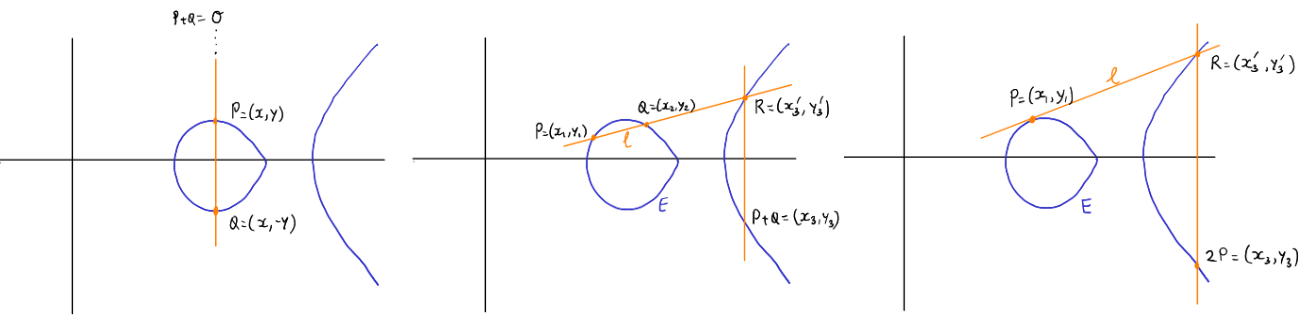
\includegraphics[width=\textwidth]{Images/ec_group_law.png}
\end{center}
One of the most interesting facts about elliptic curves is that the above 
defined geometric sum of points indeed turns the set of points $E(\bbL)$ 
into an abelian group. We explicitly state this in the next theorem, and leave 
the proof as an exercise. 

\begin{thm}
    Define $\K$, $\bbL$, $E/\K$, $E(\bbL)$ and $P + Q$ as above. Furthermore, 
    for $P = (x, y) \in E(\bbL)$, define $-P = (x, -y)$ and $-{\cal O} = {\cal O}$. 
    Then $(E(\bbL), +)$ forms an abelian group. More specifically, 
    given $P, Q, R \in E(\bbL)$, we have the following properties. 
    \begin{enumerate}[(1)]
        \item $E(\bbL)$ is closed under addition: $P + Q \in E(\bbL)$. 
        \item $E(\bbL)$ is associative: $(P + Q) + R = P + (Q + R)$. 
        \item $E(\bbL)$ is commutative: $P + Q = Q + P$.
        \item $E(\bbL)$ has identity element ${\cal O}$: $P + {\cal O} = {\cal O} + P = P$.
        \item Elements in $E(\bbL)$ are invertible: $P + (-P) = (-P) + P = {\cal O}$. 
    \end{enumerate}
\end{thm}

\begin{remark}
    In our above discussion, we have assumed that elliptic curves are 
    defined over fields that are not of characteristic $2$ or $3$. Similar 
    results can still be derived for elliptic curves defined over fields 
    of characteristic $2$ or $3$. In particular, elliptic curve points form 
    a group in these cases as well. However, deriving formulas require a 
    bit more in these cases; see Section 6.7 in \cite{10.5555/1481183}. 
\end{remark}

\subsubsection{The Size of Elliptic Curve Groups}
Let $\F_p$ be a finite field of size $p$ for some prime $p$. Let $\F_q$ 
be a finite field of size $q$ as a degree $n$ extension of $\F_p$, where 
$q = p^n$ for some positive integer $n$. Recall that finite fields are 
unique up to isomorphism, so we may assume without loss of generality that 
$\F_p = \Z_p$ is the set of integers modulo $p$, and $\F_q = 
\Z_p[z]/\langle f(z) \rangle$ is the polynomial quotient ring of some 
monic irreducible polynomial $f(z)$ of degree $n$ over $\Z_p$. 

For cryptographic purposes, we are mostly interested in elliptic curves 
defined over finite fields. For an elliptic curve $E/\F_p$ defined over 
$\F_p$, the set of $\F_q$-points $E(\F_q)$ forms an abelian group based 
on our results in the previous section, so we can naturally consider 
instantiating discrete logarithm based cryptographic protocols using $E(\F_q)$.
There are many natural questions to ask here. What is the size of 
$E(\F_q)$? What is the group structure of $E(\F_q)$? How difficult is the 
discrete logarithm problem in $E(\F_q)$? 

Let's begin with the size of $E(\F_q)$. Since $E(\F_q)$ contains the 
identity element ${\cal O}$ and the non-identity elements in $E(\F_q)$ 
form a subset of $\F_q \times \F_q$, we can easily obtain the bounds 
\[ 1 \leq |E(\F_q)| \leq q^2 + 1. \] 
Our intuition gives us a better estimate than the one above. If $E/\F_p$ 
is defined by the equation $y^2 = x^3 + ax + b$, then we would expect 
$x^3 + ax + b$ to be a perfect square in $\F_q$ for half of the elements 
$x \in \F_q$. When $x^3 + ax + b$ is a perfect square, then we expect 
exactly two values $y$ to satisfy $y^2 = x^3 + ax + b$, except when 
$x^3 + ax + b = 0$, in which case the unique corresponding value is $y = 0$. 
As a result, we would expect two elliptic curve points for about 
$(q - 1)/2$ choices of $x$, one elliptic curve point for about $1$ choice of $x$,
and no elliptic curve points for about $(q - 1)/2$ choices of $x$. This gives us 
$E(\F_q) \approx q + 1$, counting the identity element ${\cal O}$. It turns 
out that Hasse's theorem confirms this intuition. More precisely, we have 
\[ (\sqrt q - 1)^2 \leq |E(\F_q)| \leq (\sqrt q + 1)^2. \] 
\newpage 

\printbibliography
\fancyhead[R]{\nouppercase\leftmark}

\end{document}